\chapter{Numerical Methods}\label{chap:2}
In this chapter, we will discuss the fundamentals of numerical methods relevant for solving the Navier-Stokes equations.
We begin the discussion of the method of weighted residuals (\S \ref{sec:methodofweightedresiduals}) and the spatial discretisation using spectral/\emph{hp} element methods in one dimension (\S \ref{sec:spectralhpelementmethods}).
This is followed by techniques for solving the Navier-Stokes equations (\S \ref{sec:numeraltechniquesforNS}), such as the velocity-correction scheme, enforcing a constant flow rate and the quasi-3D approach for semi-homogeneous domains. 
This chapter concludes with numerical techniques for performing stability analysis of the Navier-Stokes equations (\S \ref{sec:stabilityanalysisofNS}), including eigenvalue computation and edge tracking.

%%%%%%%%%%%%%%%%%%%%%%%%%%%%%%%%%%
% 3.1 METHOD OF WEIGHTED RESIDUALS
%%%%%%%%%%%%%%%%%%%%%%%%%%%%%%%%%%

\section{Method of weighted residuals}\label{sec:methodofweightedresiduals}
Spatial discretisation errors, or residuals, arise as one seeks an approximate solution of a partial differential equation (PDE).
The method of weighted residuals provides a general mathematical framework in which constraints on the residual can be applied flexibly, thereby defining the spatial discretisation scheme and its convergence properties.
We approximate the solution of PDE by considering a finite expansion of a suitable basis, to which its coefficients are sought by minimising the inner product between the PDE and a test (or weight) function.
To demonstrate this, we consider a linear partial differential equation as,
\begin{equation}\label{eq:linear_operator}
    \mathbf{L}[u(x)] = 0, \quad x \in \Omega,
\end{equation}
where $\mathbf{L}$ refers to a linear spatial differential operator subjected to some boundary conditions within the domain, $\Omega$, while $u(x)$ refers to the exact solution of $\mathbf{L}$.
Examples of PDEs with linear spatial differential operators include the Laplace equation, $\nabla^2 u = 0 $, the Poisson equation, $\nabla^2 u - f = 0$, and the Helmholtz equation, $\nabla^2 u - \lambda u  + f = 0$.
We suppose that the exact solution $u(x)$ can be approximated (discretised) by $N$ finite number of global basis (or expansion) functions, $\Phi(x)$.
\begin{equation}\label{eq:approximate}
    u(x) \approx u^\delta(x) = \sum_{i=0}^{N-1} \hat{u}_i \Phi_i(x),
\end{equation}
where $u^\delta(x)$ refers to the approximate solution of $u(x)$, consisting of a linear combination of the product between the $i^{th}$ basis coefficient, $\hat{u}_i$, and the $i^{th}$ global basis expansion, $\Phi_i(x)$, defined within $\Omega$.
Since $u^\delta(x)$ is an approximate solution of equation \eqref{eq:helmholtz}, we expect a residual (or error) between the exact solution, $u(x)$, and $u^\delta(x)$,
\begin{equation}\label{eq:residual}
    \mathbf{L}[u^\delta(x)] = R[u^\delta(x)],
\end{equation}
where $R[u^\delta(x)]$ refers to the residual which depends on the approximate solution $u^\delta(x)$ and varies within $\Omega$.
In other words, equation \eqref{eq:residual} might not be satisfied everywhere in $\Omega$. 
Next, we need to place restrictions on the residual, such that the residual approaches zero, $R \rightarrow 0$, and the approximate solution approaches the exact solution, $u^\delta(x) \rightarrow u(x)$.
The method of weighted residuals places a restriction on the residual by applying an inner product between the governing equation and $N$ test (or weight) functions, $v_j(x)$, and setting it to zero,
\begin{equation}\label{eq:weightinnerresidual}
    (v_j(x), R[u^\delta(x)]) = 0, \quad j = 0, ..., N-1.
\end{equation}
\begin{definition}[Inner product]
The inner product between two functions $f(x)$ and $g(x)$ is,
\begin{equation}
       (f, g) = \int_\Omega f(x) g(x) dx \nonumber.
\end{equation}
\end{definition}
By enforcing equation \eqref{eq:weightinnerresidual}, the discrete problem becomes a system of $N$ ordinary differential equations to solve for the $N$ basis coefficients, $\hat{u}_i$.
The choice of test function defines the projection methods, and examples of different projection methods are shown in table \ref{tab:weightFunction}.
We emphasise that the method of weighted residuals only describes the projection method, but does not specify the type of basis expansions, as we will discuss later in \S \ref{sec:spectralhpelementmethods}.
The choice of projection method, coupled with appropriate basis expansions, will yield different convergence properties of the solution.
Of particular interest is how quickly the residual vanishes as the number of basis expansions increases.
For instance, by considering the Galerkin method coupled with Fourier expansions, one can expect exponential convergence for a sufficiently smooth problem, which is desirable for an efficient representation of turbulent dynamics.
\renewcommand{\arraystretch}{1.5} % Default value: 1
\begin{table}[h]
    \centering
        \begin{tabular}{cc}
            Weight functions & Projection method \\
            \hline
            $v_j(x) = \delta(x-x_j)$ & Collocation \\
            $v_j(x) =\left\{\begin{array}{ll}
                1 & \mbox{if } x \in \Omega_j\\
                0 & \mbox{if } x \notin \Omega_j \\
           \end{array}\right. $& Finite-Volume \\
            $v_j(x) = \phi_j$& Galerkin \\
            $v_j(x) = \frac{\partial R}{\partial \hat{u}_j}$ & Least-squares \\
            \hline
        \end{tabular}
        \caption{Examples of weight functions and projection methods}
    \label{tab:weightFunction}
\end{table}
\section{Galerkin Projection}\label{sec:galerkinprojection}
Galerkin projection remains a standard projection method in the context of finite element methods, in which the test functions, $v(x)$, are chosen to lie in the same functional space as the global basis functions, $\Phi(x)$.
To demonstrate the Galerkin projection method, we consider that the differential operator earlier in equation \eqref{eq:linear_operator} is a 1D Helmholtz equation,
\begin{subequations}\label{eq:helmholtz}
    \begin{equation}
        \mathbf{L}[u(x)] \equiv \frac{\partial^2 u(x)}{\partial x^2} - \lambda u(x) + f(x) = 0, \quad x \in \Omega := [0, l]
    \end{equation}
    \begin{equation}
        u(0) = g_D, \quad \frac{\partial u}{\partial x}\Big|_{x=l} = g_{N}.
    \end{equation}
\end{subequations}
where $\lambda$ is a real positive constant, $f(x)$ is a forcing function, and $\Omega$ refers to the spatial domain bounded between $0$ and $l$. 
To ensure that the problem is well posed, Dirichlet and Neumann boundary conditions, $g_D$ and $g_N$, are imposed at $x = 0$ and $x = l$, respectively.
Equation \ref{eq:helmholtz} is commonly referred to as the strong or classical form.

The subsequent step is to take the inner product of the equation \eqref{eq:helmholtz} with a test function, $v(x)$, that satisfies the homogeneous Dirichlet boundary conditions by definition, i.e. $v(0) = 0$, and setting the inner product to zero,
\begin{equation}\label{eq:helmholtz_inner}
    (v(x), \, \mathbf{L}[u(x)]) = \int_0^l v(x) \left[\frac{\partial^2 u(x)}{\partial x^2} - \lambda u(x) + f(x)\right] \mathrm{d}x =  0,
\end{equation}
akin to applying the method of weighted residuals (\S \ref{sec:methodofweightedresiduals}). Next, we perform integration by parts,
\begin{subequations}
    \begin{equation}\label{eq:weak_form}
        \underbrace{\int_0^l \frac{\partial v}{\partial x}\frac{\partial u}{\partial x} \, \mathrm{d}x + \int_0^l \lambda v u \, \mathrm{d}x}_{a(v,u)}= \underbrace{\int_0^l v f \, \mathrm{d}x + \left[ v \frac{\partial u}{\partial x} \right]_0^l}_{f(v)}.
    \end{equation}
    \begin{equation}\label{eq:compact}
        a(v,u) = f(v).
    \end{equation}
\end{subequations}
Equation \eqref{eq:weak_form} is typically referred to as the weak \footnote{The notions of the \emph{weak} and \emph{strong} forms refer to the smoothness (regularity) required of admissible solutions. In the weak formulation, the highest derivative involved is up to first-order, so the solution space is $H^1$. This space is generally larger than that of the strong formulation, which required $u \in \mathcal{H}^2(\Omega)$. Since $H^2(\Omega) \subset H^1(\Omega)$, the weak formulation imposes a less stringent constraint on the solution space of admissible functions.} form of equation \eqref{eq:helmholtz}.
The weak form can be represented in compact notation in equation \eqref{eq:compact}, where $a(v,u)$ is bilinear and symmetric. In structural mechanics, $a(u,u)$ is commonly referred to as the \textit{strain} energy.
To ensure that the \textit{strain} energy is finite, we restrict the choice of solutions $u(x)$ to lie in the solution space,
\begin{equation}\label{eq:solution_space}
    \mathcal{U} := \{ u \, | \, u \in H^1(\Omega), u(0) = g_D \},
\end{equation}
where $u \in H^1$ refers to functions of $u$ belonging to the Sobolev space of order 1, and satisfying the Dirichlet condition, $u(0) = g_D$,  at $x = 0$.
\begin{definition}[Sobolev space]
    We define Sobolev space of order $n \geq 1$ on $\Omega$,
    \begin{equation}
        H^n(\Omega) = \{u \, | \, u \in L_2(\Omega), D^\alpha u \in L_2(\Omega), \forall \alpha : \alpha \leq n\}, \nonumber
    \end{equation}
    where $D^\alpha u$ refers to derivatives up to order $\alpha$ and $L_2(\Omega)$ refers to functions that are square integrable.
\end{definition}
\begin{definition}[$L_2$ space]
    The space $L_2(\Omega)$ refers to functions that are square integrable,
    \begin{equation}
        (u, u)_{L_2} = \int_\Omega |u(x)|^2 \, \mathrm{d}\Omega < \infty. 
    \end{equation}
\end{definition}
In other words, $H^1$ functions satisfy the condition that the integral of the square of the function and its first derivative is finite, consistent with the highest order derivative in the weak formulation of equation \eqref{eq:helmholtz_inner}.
Similarly, the space of test functions, $\mathcal{V}$, is defined as,
\begin{equation}\label{eq:test_space}
    \mathcal{V} := \{ v \, | \, v \in H^1, v(0) = 0 \},
\end{equation}
where $v \in H^1$ refers to test functions belonging to the Sobolev space of order 1, and is defined to be zero, $v(0) = 0$, on the Dirichlet boundary condition, $x = 0$.
The generalised weak form is finding $u(x) \in \mathcal{U}$, such that
\begin{equation}\label{eq:bilinear_infinite}
    a(v,u) = f(v), \quad \forall v \in \mathcal{V}.
\end{equation}
At this point, function spaces $\mathcal{U}$ and $\mathcal{V}$ contain infinitely many possible functions and equation \eqref{eq:bilinear_infinite} is therefore infinite-dimensional.
To obtain an approximate solution, $u^\delta(x)$, we restrict ourselves to finite dimensional subspaces, $\mathcal{U}^\delta \subset \mathcal{U}$, and $\mathcal{V}^\delta \subset \mathcal{V}$.
Then, the problem is to find $u^\delta \in \mathcal{U}^\delta$, such that
\begin{equation}
    a(v^\delta, u^\delta) = f(v^\delta), \quad v^\delta \in \mathcal{V}^\delta.
\end{equation}
The subspaces $u^\delta \in \mathcal{U}^\delta$ and $v^\delta \in \mathcal{V}^\delta$ are not the same (compare the Dirichlet boundary conditions of equations \eqref{eq:solution_space} and \eqref{eq:test_space}), necessary for the standard Galerkin projection procedure where they should lie in the same subspace.
To ensure that they belong to the same space, we lift the solution $u^\delta$ into two parts,
\begin{equation}
    u^\delta = u^\mathcal{H} + u^\mathcal{D}.
\end{equation}
where $u^\mathcal{H} \in \mathcal{V}^\delta$ satisfies the homogeneous Dirichlet condition (e.g. is zero on Dirichlet boundaries), belonging to the same subsapce as $v^\delta \in \mathcal{V}^\delta$, while $u^\mathcal{D} \in \mathcal{U}^\delta$ satisfies the Dirichlet boundary conditions $u^\mathcal{D}(0) = g_D$.
Finally, the standard Galerkin projection method is to solve,
\begin{equation}\label{eq:standard_galerkin}
    a(v^\delta, u^\mathcal{H}) = f(v^\delta) - a(v^\delta, u^\mathcal{D}).
\end{equation}
This concludes the classical Galerkin formulation, where we have converted a continuous PDE into a discrete problem amenable to standard direct or iterative linear solvers.
Under certain assumptions of $a$, a solution is guaranteed under the Lax-Milgram theorem \citep{bers_ix_1955}.
The order in which we perform integration by parts, followed by defining the finite solution space, is crucial.
Reversing this order can introduce jumps in the solution derivatives between the element boundaries.

%%%%%%%%%%%%%%%%%%%%%%
% SPECTRAL/HP ELEMENTS
%%%%%%%%%%%%%%%%%%%%%%

\section{Spectral/\emph{hp} element method}\label{sec:spectralhpelementmethods}
While the procedure for approximating a solution of a PDE using the classical Galerkin projection technique has been described, the spatial discretisation scheme, related to the choice of basis (and test) functions, remains undiscussed.

In this section, we introduce the spectral/\emph{hp} element method \citep{patera_spectral_1984}, a spatial discretisation scheme in which the solution domain is partitioned into a set of non-overlapping finite elements of size $h$, within which the solution is represented as a linear combination of continuous orthogonal polynomial functions up to order $P$.
This approach combines the geometric flexibility of classical finite-element methods \citep{strang_analysis_2008}, which allow complex geometries to be represented, with the exponential convergence properties of spectral methods \citep{gottlieb_numerical_1977}.
For the reasons above, the spectral/\textit{hp} element method provides an attractive framework for approximating PDE solutions at a given cost, as we shall see later.
This section is organised as follows: domain partition, standard elements, assembly process, modal and nodal expansion functions, numerical integration and differentiation, a 1D example, before concluding with error properties of the spectral/\textit{hp} element method.

%%%%%%%%%%%%%%%%%%
% DOMAIN PARTITION
%%%%%%%%%%%%%%%%%%
\subsection{Domain partition}
The first step concerns partitioning the domain into a set of finite elemental regions.
We consider an example in one dimension within $\Omega$, and partition it into a set of $N_{el}$ elements, where $\Omega^e$ refers to the elemental partitions with $1 \geq e \geq N_{el}$, such that they meet at their boundaries and do not overlap,
\begin{equation}
    \Omega = \bigcup_{e = 1}^{N_{el}} \Omega^e, \quad \text{where} \; \bigcap_{e=1}^{N_{el}} \Omega^e = \emptyset
\end{equation}
where the $e^{th}$ element is defined as,
\begin{equation}
    \Omega^e = \{x \, | \, x_{e-1} \geq x \geq x_e \}.
\end{equation}
Each element can be represented by a linear combination of orthogonal basis expansions.
The basis expansions can be either modal or nodal expansions, as we shall see later.

%%%%%%%%%%%%%%%%%%%
% STANDARD ELEMENTS
%%%%%%%%%%%%%%%%%%%
\subsection{Standard Elements}
\begin{figure}[h]
    \centering
    \includegraphics[width=\textwidth]{NumericalMethods/Figures/standard_element_3elements.pdf}
    \caption{A spectral/\emph{hp} element representation of $u(x)$, consisting of three non-overlapping finite elements, each containing a linear combination of local expansion bases of up to $P=2$.}
    \label{fig:standard_element}
\end{figure}
In general, we expect to work with non-uniform elements that may have arbitrary lengths.
To simplify the formulation, it is convenient to define a \textit{standard} element,
\begin{equation}
    \Omega_{st} = \{ \xi \, | \, -1 \geq \xi \geq 1 \},
\end{equation}
where $\Omega_{st}$ refers to the standard element defined in local coordinates, $\xi \in [-1, 1]$.
Within this standard element, the formulation of basis expansions, as well as differential and integration operations, can be carried out in the local coordinate system $\xi$, before mapping the solution back to the global domain, $x$.
We can map the standard element into any arbitrary global coordinates based on a linear mapping $\chi^e:\Omega_{st} \rightarrow \Omega$,
\begin{equation}
    x = \chi^e(\xi) = \frac{1-\xi}{2} x_e + \frac{1 + \xi}{2}x_{e+1}, \quad \xi \in \Omega_{st}
\end{equation}
which for this case has an analytical inverse, $(\chi^e)^{-1}(x)$,
\begin{equation}
    \xi = (\chi^e)^{-1}(x) = 2 \frac{x - x_{e-1}}{x_e - x_{e-1}} - 1, \quad x \in \Omega^{e}.
\end{equation}
For illustration purposes, we consider that the standard element can be represented by three local basis expansions of polynomial order of up to $P = 2$,
\begin{equation}\label{eq:def_local_expansions}
    \phi_0^e(\xi) = \frac{1 - \xi}{2}, \quad \phi_1^e(\xi) = (1 + \xi)(1 - \xi), \quad \phi_2^e(\xi) =  \frac{1 + \xi}{2},
\end{equation}
where $\phi_0^e, \phi_2^e$ and $\phi_1^e$ refer to the linear and quadratic local basis expansions of the $e^{th}$ element.
These local basis expansions is illustrated in figure \ref{fig:standard_element}.
The approximate solution is now represented as,
\begin{equation}\label{eq:local_expansions}
    u^\delta(x) = \sum_{e=1}^{N_{el}}\sum_{i=0}^P \hat{u}_i^{e}\phi^e_i(\xi).
\end{equation}
where $\hat{u}_i^e$ refers to the local expansion basis coefficients.
The approximate solution, $u^\delta(x)$, now lie within the solution space $\mathcal{U}^\delta$ defined as,
\begin{equation}
    \mathcal{U}^\delta := \left\{ u^\delta \,\middle|\, u^\delta \in H^1,\ u^\delta(\chi^e(\xi)) \in \phi_i^e(\xi), \forall i : 0 \leq i \leq P, \forall e : 1 \leq e \leq N_{el} \right\}
\end{equation}
We note that the local basis expansions shown here are not strictly orthogonal polynomials.
By modifying them with Jacobi polynomials, they may become orthogonal as $P$ increases, as shown later.

%%%%%%%%%%%%%%%%%%%%
% ASSEMBLY FUNCTIONS
%%%%%%%%%%%%%%%%%%%%

\subsection{Global assembly}\label{sec:global_assembly}
In this section, we introduce the concept of global assembly (or direct stiffness summation) which relates the global basis expansions (equation \eqref{eq:approximate}), $\Phi_i(x)$, to the local basis expansions (equation \eqref{eq:local_expansions}), $\phi_i^e(x)$, where the solution can be approximated using either formulation,
\begin{equation}
    u^\delta(x) = \sum_{i=0}^{N-1}\hat{u}_i\Phi_i(x) = \sum_{e=1}^{N_{el}}\sum_{i=0}^P \hat{u}_i^{e}\phi^e_i(\chi^e(\xi)).
\end{equation}
In general, we can represent the global and local basis coefficients each as a column vector,
\begin{equation}
    \mathbf{\hat{u}}_g = 
\begin{pmatrix}
    \hat{u}_0 \\
    \vdots \\ 
    \hat{u}_N
\end{pmatrix},
\quad 
\mathbf{\hat{u}}_l = 
 \begin{pmatrix}
     \mathbf{\hat{u}}^0 \\ 
     \vdots \\
     \mathbf{\hat{u}}^{N_{el}-1}
 \end{pmatrix},
\end{equation}
where $\mathbf{\hat{u}}^{e} = (\hat{u}_0^e, ..., \hat{u}_P^e)^T$, $\mathbf{\hat{u}}_g \in \mathbb{R}^N$, $\mathbf{\hat{u}}_l \in \mathbb{R}^{N_{loc}}$ and $N_{loc} = N_{el}(P+1)$.
As there can be more local degrees of freedom than global degrees of freedom, $ N_{loc} > N$, we need to impose some conditions on the local expansion coefficients.
One approach is to enforce $C^0$ continuity across element boundaries, known as the continuous Galerkin projection.
Following the definition of local basis expansions in equation \eqref{eq:def_local_expansions}, we can enforce the solution to be equivalent at the elemental boundary using the condition,
\begin{equation}
    \hat{u}^{e-1}_P = \hat{u}^e_0.
\end{equation}
\begin{figure}[h]
\centering
\includegraphics[width=\textwidth]{NumericalMethods/Figures/standard_element_3elements_C0.pdf}
\caption{A graphical representation of $C^0$ across elemental boundaries and the relationship between local basis coefficients, $u_0^e, u_P^e$, and global basis expansions, $u_i$.}
\label{fig:local_to_global}
\end{figure}
The graphical representation of this condition enforcing $C^0$ continuity between the element boundaries for three finite elements with $P=2$ local basis expansions, and the relationship between global and local basis coefficients are shown in figure \ref{fig:local_to_global}.
We can relate the global and local basis coefficients with an assembly matrix, $\mathbf{A} \in \mathbb{R}^{N_{loc} \times N}$,
\begin{equation}
    \mathbf{\hat{u}}_l = \mathbf{A} \mathbf{\hat{u}}_g.
\end{equation}
In the case of $P=2$ and three finite elements ,as in the case of figures \ref{fig:standard_element}and \ref{fig:local_to_global}, the assembly matrix and the vectors of global and local basis coefficients are given as,
\begin{equation}
    \begingroup
    \setlength\arraycolsep{2pt}
    \renewcommand{\arraystretch}{1} % Smaller line spacing
        \mathbf{\hat{u}}_l = 
        \begin{pmatrix}
            \hat{u}_0^1  \\
            \hat{u}_1^1  \\
            \hat{u}_2^1  \\
            \hat{u}_0^2  \\
            \hat{u}_1^2  \\
            \hat{u}_2^2  \\
            \hat{u}_0^3  \\
            \hat{u}_1^3  \\
            \hat{u}_2^3  \\
        \end{pmatrix},
        \quad
        \mathbf{A} = 
        \begin{pmatrix}
            1 & 0 & 0 & 0 & 0 & 0 & 0\\
            0 & 1 & 0 & 0 & 0 & 0 & 0\\
            0 & 0 & 1 & 0 & 0 & 0 & 0\\
            0 & 0 & 1 & 0 & 0 & 0 & 0\\
            0 & 0 & 0 & 1 & 0 & 0 & 0\\
            0 & 0 & 0 & 0 & 1 & 0 & 0\\
            0 & 0 & 0 & 0 & 1 & 0 & 0\\
            0 & 0 & 0 & 0 & 0 & 1 & 0\\
            0 & 0 & 0 & 0 & 0 & 0 & 1\\
        \end{pmatrix}
        ,
        \quad 
        \mathbf{\hat{u}}_g
        \begin{pmatrix}
            \hat{u}_0  \\
            \hat{u}_1  \\
            \hat{u}_3  \\
            \hat{u}_4  \\
            \hat{u}_5  \\
            \hat{u}_6  \\
        \end{pmatrix},
    \endgroup
\end{equation}
The assembly matrix $\mathbf{A}$ `scatters' the global degrees of freedom to local degrees of freedom, while the transpose of it, $\mathbf{A}^T$, performs the reverse, referred to as global assembly.
For example, we wish to perform integration in the domain $\Omega$, 
\begin{equation}
    \mathbf{I}_g[j] = (\Phi_j(x), u^\delta(x)),
\end{equation}
where $\mathbf{I}_g \in \mathbb{R}^{N}$ refers to a vector containing the integral between $\Phi_i(x)$ and $u^\delta(x)$.
This is related to first performing integration using local expansion basis within standard elements, and then assembling using $\mathbf{A}^T$,
\begin{subequations}
    \begin{equation}
        \mathbf{I}_g = \mathbf{A}^T \mathbf{I}_l,
    \end{equation}
    \text{where,}
    \begin{equation}
    \mathbf{I}_g =  
    \begin{bmatrix}
        \mathbf{I}_0 \\
        \vdots \\
        \mathbf{I}_{N_g-1}
    \end{bmatrix}
    ,
    \quad 
    \mathbf{I}_l =  
    \begin{bmatrix}
        \mathbf{I}^0 \\
        \vdots \\
        \mathbf{I}^{N_{el}-1}
    \end{bmatrix}
    ,\quad \text{with} \quad
    \mathbf{I}^e =  
    \begin{bmatrix}
        \int_{-1}^1 \phi_0^e(\xi) u(\chi^e)\frac{\mathrm{d} \chi^e}{\mathrm{d} \xi}\, \mathrm{d}\xi \\
        \vdots \\
        \int_{-1}^1 \phi_{P-1}^e(\xi) u(\chi^e)\frac{\mathrm{d} \chi^e}{\mathrm{d} \xi}\, \mathrm{d}\xi
    \end{bmatrix},
    \end{equation}
\end{subequations}
and $\mathbf{I}_l \in \mathbb{R}^{N_{loc}}$ refer to the vector of integration operations performed within a standard element.
In the spectral/\textit{hp} element approach, we perform integration and differentiation using local basis expansions within a standard element.
After doing so, we assemble the local operations from the standard element to the global domain by using $\mathbf{A}^T$, as we shall show later using a 1D example.
We note that the structure of the assembly matrix is generally sparse, where the entries either contain 0, 1 or -1 in multidimensional formulation.
Therefore, the assembly matrix is not constructed in practice, and a mapping array is used instead.

%%%%%%%%%%%%%%%%%
% BASIS FUNCTIONS
%%%%%%%%%%%%%%%%%

\subsection{Local basis expansions}
The choice of local basis expansions, $\phi_i^e(\xi)$, concerns the representation of the solution, and the convergence properties of the numerical solver, in particular, the condition number of the mass and Laplacian matrices.
In general, the local basis expansions can be classified into two groups, either \textit{modal} or \textit{nodal} expansions.

% Modal expansions
\subsubsection{Modal expansions}\label{sec:nm_modalexpansions}
Modal expansions, or hierarchical expansions, describes a set of expansion basis where an expansion set ($\mathcal{X}_{P-1}^\delta$) of order $P-1$, is contained within a set ($\mathcal{X}_P^\delta$) of order $P$, e.g. $\mathcal{X}_{P-1}^\delta \subset \mathcal{X}_P^\delta$.
An example of modal expansions is the Jacobi polynomials, $P_p^{\alpha,\beta}(x)$, representing a family of solutions to the Sturm-Liouville problem within $x \in [-1, 1]$.
The Jacobi polynomials become symmetric for $\alpha = \beta$, referred to as ultraspherical polynomials. 
Special cases of ultraspherical polynomials are the Legendre polynomials, $\alpha = \beta = 1$, and the Chebyshev polynomials, $\alpha = \beta = 1/2$.
Within the Nektar++ framework, we utilise the \emph{modified} basis, based on Jacobi polynomials that are modified (hence the name),
% are used as the \emph{trial} functions. Using $\alpha=1$, $\beta=1$, and linear basis functions as \emph{boundary} modes, the modified Jacobi polynomials are,
\renewcommand{\arraystretch}{1.5} % Default value: 1
\begin{equation}\label{eq:modifiedJacobi}
    \phi_p(\xi) \rightarrow \psi_p(\xi) = \left\{
            \begin{array}{ll}
                \frac{1-\xi}{2} & \mbox{for } p=0\\
                \left(\frac{1-\xi}{2}\right)\left(\frac{1+\xi}{2}\right)P_{p-1}^{1,1}(\xi) & \mbox{for }  0 < p < P \\
                \frac{1+\xi}{2} & \mbox{for } p=P,
           \end{array}\right.
\end{equation}
We note that $\phi_p(\xi)$ refers to a general local expansion basis while $\psi_p(\xi)$ refers to the definition of the modified basis.
\begin{figure}
    \centering
    \includegraphics[width=\textwidth]{NumericalMethods/Figures/modifiedBasis_1D.pdf}
    \caption{The modified basis for up to $P=5$ normalised to $-1 \leq \psi_p \leq 1$.}
    \label{fig:modified_basis}
\end{figure}
The one-dimensional expansion modes of the modified basis of up to $P=5$ is shown in figure \ref{fig:modified_basis}.
The linear modes, corresponding to $p = 0$ and $p = P$, are the only expansions that have a magnitude at the boundaries, referred to as boundary modes.
The modified basis for $0 < p < P$ is hierarchical and has non-zero values except at the boundaries, referred to as interior/bubble modes.
Decomposing the local expansions into interior and boundary modes essentially via a partition of unity ensures that the linear modes, $P=1$, support the $C^0$ continuity across element boundaries.
So strictly speaking, the modified basis is only modal for $P>1$.

% Nodal expansions
\subsubsection{Nodal expansions}
Nodal expansions are basis expansions that are non-hierchical, $\mathcal{X}_{P-1}^\delta \not\subset \mathcal{X}_P^\delta$.
An example of nodal expansions is the Lagrange polynomials,
\begin{equation}
    \phi_p(\xi) \rightarrow h_p(\xi) = \frac{\prod_{q = 0, q \neq p}^P (\xi - \xi_q)}{\prod_{q = 0, q \neq p}^P (\xi_p - \xi_q)}
\end{equation}
The Lagrange polynomials, $h_p(\xi)$, are particularly attractive as it has a unit value at discrete nodal values, $\xi_q$, and zero everywhere else, $h_p(\xi_q) = \delta_{pq}$, which implies that
\begin{equation}
    u^\delta(\xi_q) = \sum_{p=0}^{P} \hat{u}_ph_p(\xi_q) = \sum_{p=0}^{P} \hat{u}_p\delta_{pq} = \hat{u}_q,
\end{equation}
where the Lagrange coefficient $\hat{u}_q$ is the same as the value evaluated at the node $\xi_q$.
The nodal values, $\xi_q$, are based on the Gauss-Lobatto-Legendre (GLL) points, which will be defined later in \S \ref{sec:Gaussian_quadrature}.
The nodal distribution based on GLL points is crucial for obtaining well-behaved Lagrange polynomials, as the use of equispaced nodal points leads to oscillations between nodes.
Figure \ref{fig:Lagrange_basis} presents Lagrange expansions evaluated along the GLL points.
\begin{figure}[h]
    \centering
    \includegraphics[width=\textwidth]{NumericalMethods/Figures/Lagrange_1D.pdf}
    \caption{Lagrange polynomials for $P = 5$ with nodal values along GLL points.}
    \label{fig:Lagrange_basis}
\end{figure}
\subsubsection{Multi-dimensional expansions}
We have introduced modal and nodal expansions in one dimension, and their extension to multi-dimensional bases can be generalised using a tensorial expansion of the local expansion bases. 
The standard element in a two dimensional quadrilateral, $\mathcal{Q}^2$, and a three dimensional hexahedral $\mathcal{H}^3$, are given as,
\begin{equation}
    \mathcal{Q}^2 = \{-1 \leq \xi_1, \xi_2 \leq 1 \}, \quad \mathcal{H}^2 = \{-1 \leq \xi_1, \xi_2, \xi_3 \leq 1 \}
\end{equation}
where $\xi_1, \xi_2, \xi_3$ refers to the local coordinates in multi-dimensions.
Thus, the multi-dimensional expansion bases for quadrilaterals and hexadrals using modified bases are simply a tensor product of the one-dimensional modified bases,
\begin{equation}
    \phi_{pq}(\xi_1, \xi_2) =\psi_q(\xi_1)\psi_q(\xi_2), \quad \text{and} \quad
    \phi_{pqr}(\xi_1, \xi_2, \xi_3) =\psi_q(\xi_1)\psi_q(\xi_2)\psi_r(\xi_3).
\end{equation}
\begin{figure}[h]
    \centering
        \includegraphics[width=\textwidth]{NumericalMethods/Figures/modifiedBasis.pdf}
        \caption{Two dimensional modified basis with $p = q = 4$ in a standard quadrilateral, $-1 \leq \xi_1,\xi_2 \leq 1$. The modified bases are normalised to $-1 \leq \phi_{pq} \leq 1$.}
        \label{fig:TensorialModifiedbasis}
\end{figure}
An example of the modal tensorial bases, for $p = q = 4$ in a standard quadrilateral element in shown in figure \ref{fig:TensorialModifiedbasis}.
While we have discussed the tensorial expansions for regular domains such as the standard quadrilateral and hexahedral elements, the extensions for simplex domains such as triangles, tetrahedra, prisms, and pyramids commonly used to represent complex geometries are less straightforward.
The challenge for simplexes is that the local coordinates, $\xi_1,\xi_2,\xi_3$, become dependent, where a direct tensorial expansion becomes unwieldy.
Instead, a collapsed coordinate system is introduced, providing a transformation from a standard simplex element to a standard regular element.
In this thesis, we utilise quadrilateral elements.
The reader is referred to \citet{karniadakis_spectralhp_2005} for more details about the multi-dimensional formulation of regular and simplex elements.

%%%%%%%%%%%%%%%%%%%%%%%%%%%
% NUMERICAL Integration
%%%%%%%%%%%%%%%%%%%%%%%%%%%
\subsection{Gaussian quadrature}\label{sec:Gaussian_quadrature}
In the Galerkin formulation, we routinely perform integration over the basis functions and therefore seek an efficient numerical technique.
Suppose we want to approximate the integral of a function, $u(\xi)$, in a standard element numerically given as,
\begin{equation}\label{eq:discrete_integral}
    \int_{-1}^1 u(\xi) \; \mathrm{d}\xi = \sum_{i=0}^{Q-1} w_i u(\xi_i) + R(u).
\end{equation}
The premise is determine the optimal number of quadrature points, $Q$, integration weights, $w_i$, and zeros, $\xi_i$, in which the integral error, $R(u)$, can be minimised.
If $u(\xi)$ is of polynomial order of $P$, we may expect that we require at least $P+1$ equipspaced points to represent $u(\xi)$ sufficiently.
Using Gaussian quadrature rules, we can approximate an integral of a function of order $P$, with far fewer than $P+1$ points, with specific integration weights and zeros.
In general, Gaussian quadrature rules can be grouped into three categories: Gauss, Gauss-Radau and Gauss-Lobatto quadrature.
The main difference between the three categories is in the inclusion of the endpoints.
The Gauss quadrature rule evaluates the integral without the endpoints $\xi = \pm 1$.
The Gauss-Radau quadrature rule either selects one of the endpoints, often at $\xi = -1$.
The Gauss-Lobatto quadrature rule considers both endpoints.
We will only focus on describing the Gauss-Lobatto quadrature rules and the zeros of Jacobi polynomials, known as the Gauss-Lobatto-Jacobi quadrature rules, given as,
\begin{subequations}\label{eq:weightsnzeros}
    \begin{equation}
        \xi_i^{\alpha,\beta} = \begin{cases}
            -1 \quad & i = 0, \\
            \xi_{i-1,Q-2}^{\alpha+1, \beta+1} \quad & i = 1, ..., Q-2,\\
            1, \quad & i = Q-1,
        \end{cases}
    \end{equation}
    \begin{equation}
        w_i^{\alpha,\beta} = \begin{cases}
            (\beta + 1) C_{0,Q-2}^{\alpha, \beta}, \quad & i = 0, \\
            C_{i,Q-2}^{\alpha,\beta}, \quad & i = 1, ..., Q-2, \\
            (\alpha + 1) C^{\alpha,\beta}_{Q-1,Q-2}, \quad & i = Q - 1,
        \end{cases}
    \end{equation}
    \begin{equation}
        C_{i,Q-2}^{\alpha, \beta} = \frac{2^{\alpha+\beta+1}\Gamma(\alpha+Q)\Gamma(\beta+Q)}{(Q-1)(Q-1)!\Gamma(\alpha+\beta+Q+1)[P_{Q-1}^{\alpha,\beta}(\xi_i)]^2}
    \end{equation}
\end{subequations}
where $w_i^{\alpha,\beta}, \xi_i^{\alpha,\beta}$ are the zeros (or sometimes referred to as quadrature points), and weights of the Gauss-Lobatto-Jacobi quadrature rules, and $\Gamma$ refers to the Gamma function.
For $\alpha = \beta = 0$, the quadrature points are known as the Gauss-Lobatto-Legendre (GLL) points, typically employed for Lagrange polynomials to ensure stability.
By evaluating the discrete integral (equation \eqref{eq:discrete_integral}) using the zeros and integrations weights (equation \eqref{eq:weightsnzeros}),  we can obtain an exact integral of the function $u(\xi)$, of polynomial order $P$, with at least $Q \geq (P+3)/2$ quadrature points.

%%%%%%%%%%%%%%%%%%%%%%%%%%%
% NUMERICAL DIFFERENTIATION
%%%%%%%%%%%%%%%%%%%%%%%%%%%

\subsection{Numerical differentiation}
In the same fashion as Gaussian quadrature rules, we want to evaluate the derivative of a function, $u^\delta(\xi)$, numerically.
Suppose that we want to differentiate in $x$ using local coordinates given as,
\begin{equation}
    \frac{\mathrm{d} u^\delta(\xi)}{\mathrm{d} x} = \frac{\mathrm{d} u^\delta(\xi)}{\mathrm{d} \xi}\frac{\mathrm{d} \xi}{\mathrm{d} x} = \sum_{p = 0}^P \hat{u}_p \frac{\mathrm{d} \phi_p(\xi)}{\mathrm{d}\xi}\frac{\mathrm{d}\xi}{\mathrm{d} x},
\end{equation}
where $\mathrm{d}\xi/\mathrm{d}x$ is the jacobian.
The primary step involves evaluating the derivative of the local expansion bases, $\mathrm{d} \phi_p(\xi) / \mathrm{d} \xi$.
By exploiting the Kronecker delta property of Lagrange polynomials, any polynomial can be conveniently represented by a sum of Lagrange polynomials.
Suppose that the solution has polynomial order $P$, we can represent it exactly with $P+1$ Lagrange polynomials, $\phi_p(\xi) \rightarrow h_p(\xi)$.
Its derivative through $Q \geq P + 1$ discrete nodal points, $\xi_i$ for all $i = 0, 1, \ldots, Q-1$, is expressed as,
\begin{equation}
    \frac{\mathrm{d} u ^\delta (\xi)}{\mathrm{d} \xi}\Big |_{\xi = \xi_i} = \sum_{j=0}^{P} \hat{u}_j \frac{\mathrm{d} h_j(\xi)}{\mathrm{d} \xi} \Big|_{\xi = \xi_i} = \sum_{j = 0}^{P} d_{ij}\hat{u}_j,
\end{equation}
where $\mathbf{D} = [d_{ij}] \in \mathbb{R}^{Q \times Q}$ refers to the differential matrix containing values of the derivative of the Lagrange polynomials at the quadrature points. 
Since we are evaluating the derivative along nodal (collocated) points, it is referred to as \textit{collocation} differentiation.
The general form for collocation differentiation based on Lagrange polynomials can be expressed as,
\begin{equation}\label{eq:differential_matrices}
    d_{ij} = \frac{\mathrm{d} h_j (\xi)}{\mathrm{d} \xi}\Big|_{\xi = \xi_i} = 
    \begin{cases} 
    \frac{g'_Q(\xi_i)}{g'_Q(\xi_j)} \frac{1}{\xi_i - \xi_j}, \quad & i \neq j, \\
    \frac{g''_Q(\xi_i)}{2g'_Q(\xi_i)}, \quad & i = j,
    \end{cases}
    \quad\quad
    g_Q(\xi) = \prod_{j=0}^{Q-1}(\xi - \xi_j).
\end{equation}
Since  $d_{ij}$ only depends on the choice of zeros, alternative forms of $g_q'(\xi_j)$ and $g_q''(\xi_j)$ for a choice of zeros can be found in Appendix C of \citet{karniadakis_spectralhp_2005}.
To perform collocation differentiation using a modal basis such as the modified basis, $u^\delta(\xi)= \sum_{j = 0} ^ P \hat{u}_i \psi_i(\xi)$, we need to represent the solution in nodal coordinates,
\begin{equation}
    \frac{\mathrm{d} u^\delta(\xi)}{\mathrm{d} \xi}\Big|_{\xi = \xi_i} = \frac{\mathrm{d}}{\mathrm{d} \xi}\sum_{j = 0}^P \hat{u}_j \psi_j(\xi) \Big|_{\xi = \xi_i} = \mathbf{D}\mathbf{B}\mathbf{\hat{u}},
\end{equation}
where $\mathbf{B} \in \mathbb{R}^{Q \times (P+1)}$ refers to the standard matrix which transforms the solution from coefficient space, $\mathbf{\hat{u}} \in \mathbb{R}^{P+1}$, to nodal space, $\mathbf{u} \in \mathbb{R}^{Q}$, known as the backwards transform operation, $\mathbf{u} = \mathbf{B}\mathbf{\hat{u}}$.

%%%%%%%%%%%%%%%
% EXAMPLE IN 1D
%%%%%%%%%%%%%%%

\subsection{Example in 1D}
We have outlined the basic formulation of spectral/\emph{hp} element methods in a single dimension.
To conclude the section on spectral/\textit{hp} element methods, we will describe its solution procedure, converting the weak form of the Helmholtz equation into a system of linear equations, and introduce the mass and Laplacian matrices.
Starting from the weak form,

\begin{subequations}
\begin{equation}\label{eq:example_weak_form}
    \lambda \int v u \, \mathrm{d}x + \int \frac{\partial v}{\partial x}\frac{\partial u}{\partial x} \, \mathrm{d}x = \int v f \, \mathrm{d} x + \left[v \frac{\mathrm{d} u}{\mathrm{d} x} \right]_0^l, \quad x \in [0, l],
\end{equation}
with boundary conditions,
\begin{equation}\label{eq:example_weak_form_bc}
    u(0) = g_D, \qquad \frac{\mathrm{d} u}{\mathrm{d} x}\Big|_{x=l} = g_N.
\end{equation}
\end{subequations}

We wish to seek the approximate solution $u(x) \approx u^\delta(x)$.
Suppose they can be discretised by spectral/\textit{hp} elements with $N_{el}$ elements and $P+1$ local expansion basis,
\begin{subequations}
\begin{equation}
    u^\delta(x) = \sum_{i=0}^N \hat{u}_i\Phi_i(x) = \sum_{e=1}^{N_{el}}\sum_{i=0}^P \hat{u}_i^e\phi_i^e(\xi),
\end{equation}
with test functions similarly defined as,
\begin{equation}
    v^\delta(x) = \sum_{i=0}^{N} \hat{v}_i\Phi_i(x) = \sum_{e=1}^{N_{el}}\sum_{i=0}^P \hat{v}_i^e\phi_i^e(\xi)
\end{equation}
\end{subequations}
Substituting the expansions of $u^\delta, v^\delta$ into the weak form (equation \eqref{eq:example_weak_form}) and evaluating the first term on the left-hand side using numerical quadrature over $Q$ quadrature points within a standard region,
the $e^{th}$ elemental contribution becomes,
\begin{align}
    \int_{-1}^1 \sum_{i = 0}^{P}\hat{v}^e_i\phi^e_i(\xi) \sum_{j = 0}^{P}\hat{u}^e_j\phi^e_j(\xi) \, \frac{\mathrm{d} \chi^e}{\mathrm{d} \xi} \, \mathrm{d}\xi &= \sum_{e=0}^{N_{el}-1}\sum_{q=0}^{Q-1} \left[ \sum_{i = 0}^{P}\hat{v}_i^e\phi_i^e(\xi_q) \sum_{j = 0}^{P}\hat{u}^e_j\phi_j^e(\xi_q) \right]J^e w_q^e\\ \nonumber
 & = (\mathbf{\hat{v}}^e)^T (\mathbf{B}^e)^T \mathbf{W}^e \mathbf{B}^e \mathbf{\hat{u}}^e \\ \nonumber
& = \mathbf{\hat{v}}^T \mathbf{M}^e \mathbf{\hat{u}}^e
\end{align}
where the elemental mass matrix is defined as 
\begin{equation}
    \mathbf{M}^e = (\mathbf{B}^e)^T \mathbf{W} \mathbf{B}^e \in \mathbb{R}^{(P+1)\times(P+1)}.
\end{equation}
Here, $\mathbf{B}^e \in \mathbb{R}^{Q \times (P+1)}$ refers to the elemental basis matrix, and $\mathbf{W}^e\in \mathbb{R}^{Q \times Q}$, the elemental weight matrix, a diagonal matrix consisting of the product between integration weights, $w_q^e$, and the element's jacobian, $J^e = \frac{\mathrm{d} \chi^e}{\mathrm{d} \xi}$.
\begin{equation}
    \mathbf{B}^e = 
    \begin{bmatrix}
        \phi_0^e(\xi_0) & \cdots & \phi_P^e(\xi_0) \\
        \vdots & \ddots & \vdots \\
        \phi_0^e(\xi_Q) & \cdots & \phi_P^e(\xi_Q) \\
    \end{bmatrix}
    ,
    \quad
    \mathbf{W}^e = 
    \begin{bmatrix}
        w_0^eJ^e &  & 0 \\
         & \ddots &  \\
        0 & & w_{Q-1}^eJ^e  
    \end{bmatrix}
\end{equation}
Next, we evaluate the $e^{th}$ elemental contribution of the second term on the left-hand side, 
\begin{align}
    \int_{-1}^1 \sum_{i = 0}^{P}\hat{v}^e_i\frac{\mathrm{d} \phi^e_i}{\mathrm{d} \xi} \sum_{j = 0}^{P}\hat{u}^e_j\frac{\mathrm{d} \phi^e_j}{\mathrm{d} \xi} \, \left( \frac{\mathrm{d} \chi^e}{\mathrm{d} \xi} \right)^{-1} \, \mathrm{d}\xi &= \sum_{e=0}^{N_{el}-1} \sum_{q=0}^{Q} \left[ \sum_{i = 0}^{P}\hat{v}^e_i{D}_{qi}^e\phi^e_i(\xi_q) \sum_{j = 0}^{P}\hat{u}^e_j{D}^e_{qj}\phi_j^e(\xi_q) \right]\frac{w_q^e}{J^e} \\ \nonumber
                                                                                                                                                                                                                                                  & = (J^e)^{-1}\mathbf{\hat{v}}^T (\mathbf{B}^e)^T (\mathbf{D}^e)^T \mathbf{W}^e \mathbf{D}^e \mathbf{B}^e \mathbf{\hat{u}}^e \\ \nonumber
                                                                                                                                                                                                   & = (J^e)^{-1}\mathbf{\hat{v}}^T \mathbf{L}^e \mathbf{\hat{u}}^e
\end{align}
where the elemental Laplacian matrix is defined as 
\begin{equation}
    \mathbf{L}^e = (J^e)^{-1}(\mathbf{B}^e)^T(\mathbf{D}^e)^T  \mathbf{W} \mathbf{D}^e \mathbf{B}^e \in \mathbb{R}^{(P+1)\times(P+1)},
\end{equation}
and $\mathbf{D}^e \in \mathbb{R}^{Q \times Q}$ refers to the differential matrix defined in equation \eqref{eq:differential_matrices}.
Moving onto the first term on the right hand side,
\begin{align}
    \int_{-1}^1 \sum_{i = 0}^P \hat{v}_i^e\phi_i^e(\xi) f^e(\xi) \, \frac{\mathrm{d} \chi^e}{\mathrm{d} \xi} \, \mathrm{d}\xi & = \sum_{q=0}^P \sum_{i = 0}^P \hat{v}_i^e \phi_i^e (\xi_q) f^e(\xi_q) J^e w_q^e, \\ \nonumber
                                                                                & = \mathbf{\hat{v}}^T (\mathbf{B}^e)^T\mathbf{W}^e \mathbf{f}^e \\ \nonumber
                                                                                & = \mathbf{\hat{v}}^T \mathbf{\hat{f}}^e,
\end{align}
where $\mathbf{\hat{f}}^e$ is the elemental forcing vector.
By assembling all elemental contributions, $1 \leq e \leq N_{el}$, we obtain the local system of linear equations,
  
\begin{subequations}\label{eq:local_discrete}
\begin{equation}
    \begin{bmatrix}
        \begin{bmatrix}
            \lambda \mathbf{M}^1 + \mathbf{L}^1
        \end{bmatrix} & \cdots & \mathbf{0} \\
        \vdots & \ddots & \vdots \\
        \mathbf{0} & \cdots &
        \begin{bmatrix}
            \lambda \mathbf{M}^{N_{el}} + \mathbf{L}^{N_{el}}
        \end{bmatrix} \\
    \end{bmatrix}
    \begin{bmatrix}
        \mathbf{\hat{u}}^1 \\
        \vdots  \\
        \mathbf{\hat{u}}^{N_{el}}
    \end{bmatrix}
     = 
    \begin{bmatrix}
        \mathbf{\hat{f}}^1 \\
        \vdots  \\
        \mathbf{\hat{f}}^{N_{el}}
    \end{bmatrix}
\end{equation}
or in compact form,
\begin{equation}
    [\lambda \mathbf{M}_l + \mathbf{L}_l ]\mathbf{\hat{u}}_l = \mathbf{\hat{f}}_l.
\end{equation}
\end{subequations}
where $\mathbf{M}_l \in \mathbb{R}^{N_{el}(P+1) \times N_{el}(P+1)}, \mathbf{L}_l\in \mathbb{R}^{N_{el}(P+1) \times N_{el}(P+1)}, \mathbf{\hat{u}}_l\in \mathbb{R}^{N_{el}(P+1)}$ and $\mathbf{\hat{f}}_l \in \mathbb{R}^{N_{el}(P+1)}$ refers to the local mass matrix, local laplacian matrix, vector of local expansion coefficients and local forcing vector.
To enforce $C^0$ continuity across elemental boundaries, we pre-multiply equation \eqref{eq:local_discrete} with the assembly map, $\mathbf{A}^T$, and express local coefficients as global coefficients,
\begin{equation}
    \mathbf{A}^T[\lambda \mathbf{M}_l + \mathbf{L}_l]\mathbf{A} \mathbf{\hat{u}}_g = \mathbf{A}^T \mathbf{\hat{f}}.
\end{equation}
Finally, we consider the boundary conditions by lifting $u^\delta(x) = u^\mathcal{H}(x) + u^\mathcal{D}(x)$
\begin{equation}
    \mathbf{A}^T[\lambda \mathbf{M}_l + \mathbf{L}_l]\mathbf{A} \mathbf{\hat{u}^\mathcal{H}}_g = \mathbf{A}^T \mathbf{\hat{f}} + \mathbf{A}^T[\lambda \mathbf{M}_l - \mathbf{L}_l]\mathbf{A} \mathbf{\hat{u}^\mathcal{D}}_g.
\end{equation}
We then solve this system for the homogeneous coefficients $\mathbf{\hat{u}}_g^\mathcal{H}$.

\subsection{Error properties}
Suppose we consider $P+1$ orthogonal polynomials spanning the polynomial space of $\mathcal{P}_P$, the energy norm of the error, $||\varepsilon||_E = ||u(x) - u^\delta (x)||_E$\footnote{The energy norm is defined as $||u||_E = \sqrt{a(u,u)}$, where $a(u,u)$ is the bilinear operator introduced in equation \eqref{eq:compact}. It is a measure of functions belonging to the \textit{energy} space which are $H^1$ functions.} for element size of $h$ and polynomial order $P$, satisfies the convergence property \citep{babuska_p_1994},
\begin{equation}\label{eq:error_convergence}
    ||\varepsilon||_E \leq C h^{\mu - 1}P^{-(k-1)}||u||_k,
\end{equation}
where $\mu = \min (k, P+1)$, and $C$ is independent of $h, P$ and $u$.
To illustrate this convergence property, we consider the exact solution $u = \sin(\pi x)$ of the 1D Helmholtz problem on the domain $x \in [-1, 1]$ with Dirichlet boundary conditions on both ends and $\lambda = 1$.
\begin{figure}[h]
    \centering
    \includegraphics[width=\textwidth]{NumericalMethods/nektar-convergence/hp-convergence.pdf}
    \caption{Convergence properties of an exact solution $u = \sin (\pi x)$ to a 1D Helmholtz equation with $\lambda = 1$ and Dirichet boundary conditions at $x \in [-1, 1]$. $h$-type refinement is performed on a mesh with fixed $P=1$ and decreasing $h$ (increasing elements), demonstrating algebraic convergence in a \textit{log-log} plot of (a). $p$-type refinement is performed on a mesh with equi-spaced two elements and increasing $P$, demonstrating exponential convergence on a \textit{semi-log} plot of (b).}
    \label{fig:hp-convergence}
\end{figure}
This convergence property arising from the $h$- and $p$-type refinements is shown in figure \ref{fig:hp-convergence}.
    To ensure consistency between the two types of refinement, the number of degrees of freedom, $N_{dof}$, is shown on the abscissa, which scales as $\mathcal{O}(h) \sim \mathcal{O}(N_{dof}^{-1})$ and $\mathcal{O}(p) \sim \mathcal{O}(N_{dof})$.
For $h$-refinement, the number of elements is doubled on a mesh with fixed polynomial order $P=1$, demonstrating algebraic convergence, $||\varepsilon||_E \sim \mathcal{O}(h)$ in figure \ref{fig:hp-convergence}(a).
For $p$-refinement, the polynomial order $P$ is increased on a mesh with two equispaced elements, showing exponential convergence, $||\varepsilon||_E \sim \mathcal{O}(c^p)$ where $c$ is a constant, in figure \ref{fig:hp-convergence}(b).

%%%%%%%%%%%%%%%%%%%%%%%%%%%%%%%%%%%%%
% TECHNIQUES FOR SOLVING NS EQUATIONS
%%%%%%%%%%%%%%%%%%%%%%%%%%%%%%%%%%%%%

\section[Numerical methods for solving the N.S equations]{Numerical methods for solving the Navier-Stokes equations}\label{sec:numeraltechniquesforNS}
\subsection{Velocity Correction Scheme}\label{sec:nm_vcs}
The spatial discretisation of the Helmholtz operator and its numerical solution procedure have been discussed using the spectral/\emph{hp} element methods.
Here, we describe the numerical methods that are used to solve the Navier-Stokes equations given as,
\begin{subequations}
    \begin{equation}\label{eq:velocity_explicit}
    \frac{\partial u}{\partial t}  + (\mathbf{u} \cdot \nabla) \mathbf{u} = -\nabla p + \nu \nabla^2 \mathbf{u} + \mathbf{f}
\end{equation}
\begin{equation}
    \nabla \cdot \mathbf{u} = 0,
\end{equation}
\text{with boundary conditions,}
\begin{equation}
    \mathbf{u} = 0, \quad \text{on} \; \partial \Omega.
\end{equation}
\end{subequations}
In the above, the primitive variables are velocity and pressure $(\mathbf{u}, p)$, and we assumed unit density, $\rho = 1$, with the kinematic viscosity appearing as the control parameter.
The time evolution of velocity is explicitly expressed in equation \eqref{eq:velocity_explicit}, but does not appear for the pressure, which is coupled to the velocity field, enforcing the incompressibility condition.
Several strategies exist for addressing the coupled velocity-pressure fields by
\begin{enumerate}
    \item Solving the coupled system, such as the Uzawa algorithm,
    \item Splitting methods,
\end{enumerate}
We adopt splitting methods, which decompose the Navier-Stokes equations into subproblems and solve them sequentially.
These methods, which belong to the broader family of projection methods introduced by \citet{chorin_numerical_1967} and \citet{temam_sur_1969}, can be further classified as pressure-correction or velocity-correction schemes.
This thesis employs the use of the high-order velocity-correction scheme introduced by \citet{karniadakis_high-order_1991} and further explained by \citet{guermond_velocity-correction_2003}.
We rewrite the incompressible Navier-Stokes equations in semi-discrete form using linear and nonlinear operators as,
\begin{subequations}\label{eq:semidiscreteNS}
    \begin{equation}\label{eq:semidiscreteNSa}
        \frac{\partial \mathbf{u}}{\partial t} = \mathrm{\mathbf{N}(\mathbf{u})} - \nabla p +  \nu \mathrm{\mathbf{L}}(\mathbf{u}),
    \end{equation}
    \begin{equation}
        \nabla \cdot \mathbf{u} = 0,
    \end{equation}
    \text{with boundary conditions,}
    \begin{equation}
        \mathbf{u}|_\Omega = 0, \quad \mathbf{u}(t=0) = \mathbf{u}_0.
    \end{equation}
\end{subequations}
The nonlinear, $\mathbf{N}$, linear, $\mathbf{L}$, operators are obtained from a suitable spatial-discretisation method such as the spectral/\emph{hp} element method.
The nonlinear and linear operators are defined as,
\begin{equation}
    \mathrm{\mathbf{N}}(\mathbf{u}) \equiv - (\mathbf{u} \cdot \nabla)\mathbf{u}, \qquad \mathrm{\mathbf{L}}(\mathbf{u}) \equiv \nabla^2 \mathbf{u},
\end{equation}
To minimise aliasing errors in the quadratic nonlinear terms, we perform numerical integration by increasing the number of quadrature points to $Q \geq (P + 3)/2$.
To advance the velocity at time step, $\mathbf{u}^{n}$, to the next time step, $\mathbf{u}^{n+1}$, we integrate equation \eqref{eq:semidiscreteNS} over a time step $\Delta t$,
\begin{equation}\label{eq:split}
\mathbf{u}^{n+1} - \mathbf{u}^n = \underbrace{\int_{t_n}^{t_{n+1}} \mathbf{N}(\mathbf{u}) \, \mathrm{d}t}_{\Delta t \sum_{q=0}^{J_e - 1} \beta_q \mathbf{N}(\mathbf{u}^{n-q})} \; - \; \underbrace{\int_{t_n}^{t_{n+1}} \nabla p \, \mathrm{d} t}_{\Delta t \nabla \bar{p}^{n+1}} \; + \; \nu\underbrace{\int_{t_n}^{t_{n+1}} \mathbf{L}(\mathbf{u})\, \mathrm{d}t}_{\Delta t \sum_{q = 0}^{J_i - 1} \gamma_q \mathbf{L}(\mathbf{u}^{n+1-q})}.
\end{equation}
The velocity correction scheme `splits' equation \eqref{eq:semidiscreteNS} into three steps shown as underbraces, which are evaluated successively from left to right.
The first step we perform is to extrapolate the advection velocities, by approximating the nonlinear terms using an explicit scheme such as the Adams-Bashforth family of $J_e$ order,
\begin{equation}\label{eq:firstStep}
    \frac{\mathbf{\hat{u}} - \sum_{q=0}^{J_e-1} \alpha_{q} \mathbf{u}^{n-q}}{\Delta t} = \sum_{q=0}^{J_e-1} \beta_q \mathrm{\mathbf{N}}(\mathbf{u}^{n-q}),
\end{equation}
where $\mathbf{\hat{u}}$ is denotes the primary intermediate velocity field desired and $\alpha_e,\beta_e$ refers to the time integration coefficients for a prescribe $J_e$-th order, described later.
After evaluating $\mathbf{\hat{u}}$, we move onto the second term in equation \eqref{eq:split}, which defines the pressure at time step $n+1$ as,
\begin{equation}\label{eq:secondStep}
    \frac{\mathbf{\hat{\hat{u}}} - \mathbf{\hat{u}}}{\Delta t} = -\nabla p^{n+1}.
\end{equation}
$\mathbf{\hat{\hat{u}}}$ denotes as the secondary intermediate velocity.
In this single equation, we seek to obtain two unknown solutions, $\mathbf{\hat{\hat{u}}}$ and $p^{n+1}$.
The splitting method assumes that the secondary intermediate velocity is divergence free, $\nabla \cdot \mathbf{\hat{\hat{u}}} = 0$, and satisfies the Dirichlet boundary conditions normal to the boundary, $\mathbf{\hat{\hat{u}}} \cdot \mathbf{n} = \mathbf{u}|_\Omega \cdot \mathbf{n}$.
By considering the assumptions above and the divergence of equation \eqref{eq:secondStep}, we obtain the pressure Poisson equation with the primary intermediate velocity acting as the forcing term,
\begin{subequations}
    \begin{equation}\label{eq:pressurePoisson}
        \nabla^2 p^{n+1} = \nabla \cdot \left(\frac{\mathbf{\hat{u}}}{\Delta t}\right)
    \end{equation}
    \text{and boundary conditions,}
    \begin{equation}\label{eq:pressureBC}
    \frac{\partial p^{n+1}}{\partial n} = \mathbf{n} \cdot \left(\frac{\mathbf{\hat{\hat{u}}} - \mathbf{\hat{u}}}{\Delta t}\right).
    \end{equation}
\end{subequations}
While the pressure boundary condition \eqref{eq:pressureBC} is straightforward to evaluate, it is sensitive to large splitting errors \citep{karniadakis_high-order_1991}.
To overcome this, we consider a high-order boundary condition of pressure, obtained from equation \eqref{eq:semidiscreteNSa},
\begin{equation}\label{eq:modifiedpressureBC}
    \frac{\partial p^{n+1}}{\partial t} = -\sum_{q=0}^{J_e-1} \beta_q \left[ \frac{1}{\Delta t} \mathbf{u}^{n-q} + \nu [\nabla \times (\nabla \times \mathbf{u}^{n-q})] + (\mathbf{u}^{n-q} \cdot \nabla)\mathbf{u}^{n-q} \right] \cdot \mathbf{n}.
\end{equation}
Notably, the linear operator is expressed as $\mathbf{L}(\mathbf{u}) = \nabla(\nabla \cdot \mathbf{u}) - \nabla \times (\nabla \times \mathbf{u})$, where the divergence is set to zero, favouring numerical stability \citep{orszag_boundary_1986,karniadakis_high-order_1991}.
$J_e$ is the order the explicit scheme as in equation \eqref{eq:firstStep}.
After solving for the pressure Poisson equation, the secondary intermediate velocity could be subsequently obtained using equation \eqref{eq:secondStep}.
After which, we can move on to the final substep in equation \eqref{eq:split}, by solving a Helmholtz equation for $\mathbf{u}^{n+1}$, 
\begin{equation}\label{eq:thirdStep}
    \frac{\gamma_0\mathbf{u}^{n+1} - \hat{\hat{\mathbf{u}}}}{\Delta t} = \nu \sum_{q=0}^{J_i-1} \gamma_q \mathrm{\mathbf{L}}(\mathbf{u}^{n+1-q}),
\end{equation}
where the linear terms are treated based on a family of Adams-Moulton implicit schemes and $J_i, \gamma_q$ denotes the order of the scheme and time integration coefficients, completing the velocity correction scheme.
The time integration coefficients are determined from stiffly stable schemes shown in table \ref{tab:stiffyStableCoefficients}, an improvement from the Adams-family schemes \citep{karniadakis_high-order_1991}.
\renewcommand{\arraystretch}{1.} % Default value: 1
\begin{table}[h]
    \centering
        \begin{tabular}{c c c c}
            Coefficients & $1^{st}$ order & $2^{nd}$ order & $3^{rd}$ order \\
            \hline
            $\gamma_0$ & 1 & 3/2 & 11/6 \\
            $\alpha_0$ & 1 & 2   & 3    \\
            $\alpha_1$ & 0 & -1/2 & -3/2 \\
            $\alpha_2$ & 0 & 0  & 1/3 \\
            $\beta_0$ & 1 & 2 & 3 \\ 
            $\beta_1$ & 0 & -1 &  -3 \\
            $\beta_2$ & 0 & 0 &   1 \\
        \end{tabular}
        \caption{Integration coefficient of stiffly stable schemes from \cite{karniadakis_high-order_1991}.}
    \label{tab:stiffyStableCoefficients}
\end{table}
The high-order velocity correction scheme can be summarised in a three-step process of the following,
\begin{equation}
    \mathbf{u}^n \xrightarrow{\quad \mathbf{N}(\mathbf{u}^n) \quad} \mathbf{\hat{u}} \xrightarrow{\quad \nabla^2 p \quad} \mathbf{\hat{\hat{u}}} \xrightarrow{\quad \mathbf{L}(\mathbf{\hat{\hat{u}}}) \quad} \mathbf{u}^{n+1}, \nonumber
\end{equation}
evolving the velocity fields at time step $n$ to $n+1$.

%%%%%%%%%%%%%%%%%%%%%%%%%%%%%%%%%%%%%
% FOURIER SPECTRAL/HP ELEMENT METHODS
%%%%%%%%%%%%%%%%%%%%%%%%%%%%%%%%%%%%%

\subsection{Fourier spectral/\emph{hp} modes}\label{sec:nm_quasi3d}
Fourier-Chebyshev-Fourier type discretisation has been recognised as the preferred method for performing direct numerical simulations (DNS) of transitional or turbulent incompressible channel flows \citep{kim_turbulence_1987} owing to its efficient representation of the inhomogeneous wall-normal directions and the homogeneous streamwise and spanwise directions, using Chebyshev and Fourier expansions, respectively.

The Fourier spectral/\emph{hp} element method is related to this approach, where the homogeneous and the inhomogeneous directions are represented by Fourier expansions and spectral/\emph{hp} elements, respectively.
This approach is commonly referred to as the Quasi-3D (2.5D) approach, which allows the representation of a single homogeneous direction with two inhomogeneous directions.
For example, in turbulent channel flows with riblets, Fourier expansions are used to represent the periodic streamwise direction, while the spectral/\emph{hp} elements are used to discretise the spanwise and wall-normal directions.
In the analysis of three-dimensional wakes of cylinders, the span is treated via Fourier expansions.
In this thesis, we routinely use the Quasi-3D approach, consisting of 2D spectral/\emph{hp} elements with 1D Fourier expansions, which discretise the cross-stream plane and the streamwise flow, respectively. 
The velocity and pressure in the spectral/\emph{hp} plane are described by two-dimensional modified bases with Fourier expansions,
\begin{equation}\label{eq:fourierSpectral}
    \begin{bmatrix}
        \mathbf{u}^\delta(x,y,z,t) \\
        p^\delta(x,y,z,t)
    \end{bmatrix}
    =
    \sum_{k=0}^{N_z-1} \sum_{p=0}^{P} \sum_{q=0}^{P} \psi_p(x) \psi_q(y) e^{ik\beta z}
    \begin{bmatrix}
         \hat{\mathbf{u}}_{p,q,k}(t) \\
         \hat{p}_{p,q,k}(t)
    \end{bmatrix}
    =
    \sum_{k=0}^{N-1} e^{ik\beta z} \begin{bmatrix}
        \mathbf{\tilde{u}}_k(x,y,t) \\ \tilde{p}_k(x,y,t)
    \end{bmatrix}
\end{equation}
where $\beta = \frac{2\pi}{L_z}$ is the spanwise wavenumber, $L_z$ the spanwise length, $N_z$ the number of Fourier expansions.
Substituting equation \ref{eq:fourierSpectral} into the Navier-Stokes equations and taking the Fourier transform (equivalently to the Galerkin projection with respect to Fourier expansion as a test function) yields a system of $N_z$ decoupled equations, amenable to parallel processing,
\begin{subequations}\label{eq:fouriertransformedNS}
\begin{equation}
    \frac{\partial \mathbf{\tilde{u}}_k}{\partial t} = - \tilde{\nabla}_k \tilde{p}_k + \nu(\nabla^2_{x,y} - k^2\beta^2)\mathbf{\tilde{u}}_k - \widehat{\left[(\mathbf{u} \cdot \nabla) \mathbf{u}\right]}_k 
\end{equation}
\begin{equation}
    - k \beta \tilde{\nabla} \cdot \mathbf{\tilde{u}}_k = 0, \quad k = 0, ..., N_z-1
\end{equation}
\end{subequations}
where $\tilde{\nabla}_k = (\frac{\partial}{\partial x}, \frac{\partial}{\partial y}, ik\beta)$, $\nabla_{x,y}^2 = (\frac{\partial^2}{\partial x^2}, \frac{\partial^2}{\partial y^2})$ and $\widehat{\left[(\mathbf{u} \cdot \nabla) \mathbf{u} \right]_k}$ refers to the $k^{th}$ Fourier component of the nonlinear term.

\subsection{Maintaining fluid flow through a channel}\label{sec:nm_constantflux}
\begin{figure}[h]
    \centering
    \includegraphics[width=\textwidth]{NumericalMethods/Figures/flowrate.pdf}
    \caption{(a) Flow rate driven by a pressure gradient from a reservoir elevated by $h$. (b) Flow driven by a piston at a constant flow rate.}
    \label{fig:flowrate}
\end{figure}
In general, there are two approaches to drive a fluid flow through a channel, either by maintaining a constant pressure drop or a constant volumetric flux (flow rate).
This difference is illustrated in figure \ref{fig:flowrate}, whereby the flow through the channel is driven by a constant pressure drop from an elevated reservoir of constant height $h$ in figure \ref{fig:flowrate}(a), while a piston moves at a constant speed rightwards, drawing fluid through the channel at a constant volumetric flux in figure \ref{fig:flowrate}(b).
\subsubsection{Constant pressure gradient via body-forcing}
We decompose the pressure as
\begin{equation}
    p(x) = \tilde{p}(x) - f_x x,
\end{equation}
where $p, \tilde{p}, f_x$ refer to the pressure, consisting of a sum of a periodic component of pressure (i.e. $\tilde{p}(x+L_x) = \tilde{p}(x)$ where $L_x$ is the streamwise length of the computational domain) and a constant pressure gradient, respectively.
This decomposition is used when $\tilde{p}$ is represented by Fourier expansions in the homogeneous direction.
Substituting this decomposition into the streamwise component of the Navier-Stokes equations yields,
\begin{equation}\label{eq:streamwise_equation}
    \frac{\partial u}{\partial t} + (u \cdot \nabla) u = -\frac{\partial \tilde{p}}{\partial x} + \nu \nabla^2 u + f_x.
\end{equation}
The constant pressure gradient $f_x$ appears as a body force.
The central question then concerns the magnitude of the body force (or pressure gradient) required to maintain either laminar or turbulent flow.
To proceed, we decompose the streamwise velocity field into mean and fluctuating components,
\begin{equation}
    u(x,y,t) = U(y) + u'(x,y,t),
\end{equation}
where $U(y) = \langle u \rangle$ refers to the averaged velocity and $\langle \cdot \rangle = \frac{1}{TL_xL_z}\int \; \cdot \; dzdxdt$ refers to the temporal and span-averaged operator.
The fluctuating component is defined with an average of 0, i.e. $\langle u' \rangle = 0$.
Next, we substitute this decomposition into equation \eqref{eq:streamwise_equation}, and perform the averaging operation,
\begin{equation}
    \begin{split}
    & \Biggl\langle \frac{\partial (U + u')}{\partial t} + (U+u') \frac{\partial (U+u')}{\partial x} + (V + v') \frac{\partial (V + v')}{\partial y} \\
    & = -\frac{\partial (P + p')}{\partial x} + \nu\nabla^2(U + u') + F_x + f_x' \Biggr\rangle.
    \end{split}
\end{equation}
For a statistically stationary turbulent (or laminar) channel flow with periodic streamwise boundary conditions, we can make the following assumptions:
\begin{enumerate}
    \item stationary flow $\frac{\partial U}{\partial t} =  0$,
    \item fully-developed in $x$, $\frac{\partial}{\partial x} \rightarrow 0$, 
    \item $\frac{\partial V}{\partial y} = 0$, as a consequence of continuity and the no-slip boundary condition.
    \item $\langle u',v',w',p' \rangle  = 0$, based on the definition of fluctuations,
    \item $\frac{\partial \tilde{p}}{\partial x} = 0 $ due to the enforced periodicity in $x$.
\end{enumerate}
Applying the assumptions above, the mean momentum equations simplify into,
\begin{equation}
\langle F_x \rangle = \left\langle \frac{\partial (u'v')}{\partial y} \right\rangle - \nu \frac{\partial U^2}{\partial y^2},
\end{equation}
where the body force on the left-hand side balances the sum of Reynolds stresses and viscous diffusion on the right-hand side.
Next, we integrate the expression from $y \in [-1, 1]$, 

\begin{equation}
    2F_x = [\left\langle u'v'\right\rangle]_{y=-1}^{y=1} + \nu \left [\frac{\partial U}{\partial y}\biggr|_{y=1} - \frac{\partial U}{\partial y}\biggr|_{y=-1} \right].
\end{equation}
The wall shear stress is defined by $\tau_w = \nu \frac{\partial U}{\partial y}|_{y=1}$ ($\rho$ is assumed to be 1), and it is antisymmetric about the channel centreline, $\nu \frac{\partial U}{\partial y}|_{y=1} = - \nu \frac{\partial U}{\partial y}|_{y=-1}$.
Due to the no-slip condition, the Reynolds shear stress is zero, i.e. $[u'v']|_{y=-1,1} = 0$.
Hence, the expression above simplifies to,
\begin{equation}\label{eq:eq6}
    \tau_w = F_x.
\end{equation}
In other words, the body force $F_x$ is balanced by the wall shear stress (drag), $\tau_w$, along the channel walls.
In the case of laminar flow, $\tau_w$ can be determined analytically, and the body force required for sustaining a laminar flow for a velocity profile of $u(y) = 1 - y^2$, is $F_x = -2\nu$.
However, determining the wall shear stress (and hence the magnitude of the body force) is not a straightforward task for transitional or turbulent channel flow, as there is no analytical expression for $\tau_w$ and its dependence on Reynolds number.
Instead, we can only rely on the empirical relations of turbulent channel flow between the skin friction coefficient, $c_f = \tau_w / \frac{1}{2}\rho U_c^2$ and Reynolds number $Re_c$ from \citet{dean_reynolds_1978}.
\begin{equation}
    c_f = 0.00302Re_c^{-1/4},
\end{equation}
where $Re_c$ is the Reynolds number based on the laminar centerline velocity.
\begin{figure}[h]
\centering
\includegraphics[width=\textwidth]{NumericalMethods/Figures/cf-Rec.pdf}
\caption{$c_f$ against $Re_c$ using data from \cite{dean_reynolds_1978} with $\rho = U_c = 1$. Experimental scatter points from \citep{patel_observations_1969, kim_turbulence_1987, iida_relaminarization_1998, tsukahara_dns_2014}.}
\label{fig:tauw_rec}
\end{figure}
Similarly, the skin friction coefficient for the case of laminar flow is $c_f = 4/Re_c$ \citet{dean_reynolds_1978}.
Figure \ref{fig:tauw_rec} illustrates the relationship between $\tau_w$ and $Re_c$ of channel flow using the empirical relationships from \citet{dean_reynolds_1978} (here $\rho = U_c = 1$) and experimental data from \citet{patel_observations_1969,kim_turbulence_1987, iida_relaminarization_1998, tsukahara_dns_2014}.
While the empirical relationships for laminar flow, $Re_c \lesssim 1000$, and turbulent flow, $Re_c \gtrsim 2000$, appear reasonably robust, the wall shear stress in the transitional region is lacking.
Since we are investigating flow regimes in the transitional region, we will not adopt the body forcing approach.


\subsubsection{Constant volumetric flux}
An alternative approach is to enforce a constant volumetric flux, illustrated using the piston method in figure \ref{fig:flowrate}(b).
We employ the efficient Green's function approach introduced by \citet{chu_direct_1993}, and outline its solution procedure.
The volumetric flux is defined as,
\begin{equation}
    Q(\mathbf{u})=\frac{1}{A_{s}}\int_{R} \mathbf{u} \cdot \mathrm{d}\mathbf{R},
\end{equation}
where $Q(\cdot)$ refers to the flow rate operator through the surface $R$ with surface area of $A_s$.
The idea is to add a correction velocity, $\mathbf{u}_{corr}$, to the velocity field at time step $n$, $\mathbf{u}^{n}$, such that the corrected solution, $\mathbf{\bar{u}}^{n} = \mathbf{u}^{n} + \mathbf{u}_{corr}$, has the desired volumetric flux $\bar{Q}= Q(\mathbf{\bar{u}}^{n})$.
While adding two solutions is straightforward, the resulting velocity field may not satisfy the Navier-Stokes equations directly.
Fortunately, we can leverage the velocity correction scheme, which (in general) evaluates the nonlinear advection terms followed by the linear terms (pressure and dissipation).
This process is summarised as,
\begin{equation}\label{eq:two_step}
    \begin{cases} 
        \frac{\partial \mathbf{u}}{\partial t} = \mathbf{N}(\mathbf{u})\\ 
        \mathbf{u}(\mathbf{x}, 0) = \mathbf{u}^{n}
    \end{cases}
    \quad 
    \xrightarrow{\qquad \mathbf{\hat{u}}(\mathbf{x}, \Delta t) \qquad}
    \quad 
    \begin{cases} 
        \frac{\partial \mathbf{u}}{\partial t} = -\nabla p + \nu \mathbf{L}(\mathbf{u}) \\
        \mathbf{u}(\mathbf{x}, 0) = \mathbf{\hat{u}}(\mathbf{x}, \Delta t),
    \end{cases}
\end{equation}
where $\mathbf{u}(\mathbf{x},0) = \mathbf{u}^n$ and $ \mathbf{\hat{u}}(\mathbf{x}, \Delta t)$ refer to the initial condition for the nonlinear advection terms, and the intermediate velocity, the initial condition for the linear terms, respectively.
Since the second step consists of solving the linear Stokes equation, any solution of the linear Stokes (such as $\mathbf{u}_{corr}$) added to the final solution will still satisfy the linear Stokes equations - a property of linear differential equations.
We consider the linear Stokes equation governing the evolution of the correction velocity,
\begin{equation}\label{eq:alpha}
    \frac{\partial \mathbf{u}_{corr}}{\partial t} = - \nabla p_{corr} + \nu \mathbf{L}(\mathbf{u}_{corr}) + \alpha^n \mathbf{\hat{e}_x},
\end{equation} 
where $\alpha^n$ is the undetermined magnitude of body force at time step $n$ in the streamwise direction, $\mathbf{\hat{e}}_x$, required to maintain the desired flow rate $\bar{Q} = Q(\mathbf{u}^n) + Q(\mathbf{u}_{corr})$. 
Since $\mathbf{u}_{corr}$ is to be added to $\mathbf{u}^n$, the initial condition for $\mathbf{u}_{corr}$ must be $\mathbf{u}_{corr}(\mathbf{x}, 0) = 0$, so that $\mathbf{u}^n$ remains compatible with the initial conditions in equation \eqref{eq:two_step}.
Since $\alpha^n$ is undetermined, we normalise the equation with respect to $\alpha^n$, yielding the linear Stokes equations with unit forcing,
\begin{equation}\label{eq:unit_stokes}
    \frac{\partial \mathbf{v}}{\partial t} = - \nabla \hat{p} + \nu \mathbf{L}(\mathbf{v}) + \mathbf{\hat{e}_x}, \quad \mathbf{v}(\mathbf{x}, 0) = \mathbf{0}, 
\end{equation} 
where $\mathbf{v} = \mathbf{u}_{corr} / \alpha^n$ and $\hat{p}  = p_{corr} / \alpha^n$.
The corrected velocity field becomes
\begin{equation}
    \mathbf{\bar{u}} = \mathbf{u} + \alpha^n \mathbf{v}^1,
\end{equation}
where $\mathbf{v}^1$ is a solution field obtained by solving equation \eqref{eq:unit_stokes} in the first time step.
To match the target volumetric flux, $\bar{Q}$, we need to scale $\alpha^n$ such that,
\begin{equation}
    \bar{Q} = Q(\mathbf{\bar{u}}^n) =  Q(\mathbf{u}^n) + Q(\alpha^n \mathbf{v}^1).
\end{equation}
which gives,
\begin{equation}
    \alpha^n = \frac{\bar{Q} - Q(\mathbf{u}^n)}{Q(\mathbf{v}^1)},
\end{equation}
evaluated at every time step $n$.
This Green's function approach is computationally efficient because we only need to compute $\mathbf{v}^1$ and $Q(\mathbf{v} ^1)$ once in the first time step and reuse them for subsequent time steps.
The process of adding the correction velocity at the end of the velocity correction scheme can be summarised in the process as follows,
\begin{equation}
    \mathbf{u}^n \xrightarrow{\quad \mathbf{N}(\mathbf{u}^n) \quad} \mathbf{\hat{u}} \xrightarrow{\quad \nabla^2 p \quad} \mathbf{\hat{\hat{u}}} \xrightarrow{\quad \mathbf{L}(\mathbf{\hat{\hat{u}}}) \quad} \mathbf{u}^{n+1} \xrightarrow {\quad \alpha^{n+1} \mathbf{v}^1 \quad} \mathbf{\bar{u}}^{n+1} \nonumber.
\end{equation}

\section[Stability analysis of the N.S equations]{Stability analysis of the Navier-Stokes equations}\label{sec:stabilityanalysisofNS}
\subsection{Algorithms for linear stability analysis}\label{sec:nm_arnoldi}
In this section, we present a general overview of the numerical procedure for linear stability analysis.
Linear stability analysis examines the stability of a base flow by considering the evolution of infinitesimal perturbations.
In general, these perturbations may grow or decay exponentially, indicating whether the base flow is linearly unstable or stable, respectively.
In \S \ref{sec:bkgrd_transitional}, we introduced linear stability analysis in the context of wall-bounded shear flows leading to the Orr-Sommerfeld equations, where the base flows depend on a single inhomogeneous and two homogeneous directions, commonly referred to as local\footnote{Referring to being spatially local in the context of `real' flows which are typically inhomogeneous in all directions} stability analysis.
For example, the laminar Poiseuille flow, $U(y) = 1 - y^2$, and the laminar Couette flow $U(y) = y$, $y \in [-1, 1]$.
For some flows, such as boundary layers, wakes and jets, their base flows are not strictly parallel.
By considering a weak dependence on the stream and spanwise directions, their stability is described by the parabolised stability equations \citep{herbert_parabolized_1997}.
When the base flow depends on two spatially inhomogeneous directions, $U(x,y)$, or three spatially inhomogeneous directions, $U(x,y,z)$, the analysis of such states is commonly referred to as biglobal or triglobal stability analysis, respectively \citep{theofilis_advances_2003}.
If the base flow is time-dependent, such as in the secondary instability of cylinder flows, we use Floquet stability analysis \citep{henderson_secondary_1996}.

In this section, we consider a time-independent base flow and consider a generic decomposition of the velocity field in three spatial dimensions,
\begin{equation}
    \mathbf{u}(\mathbf{x}, t) = \mathbf{U}(\mathbf{x}) + \mathbf{u}'(\mathbf{x}, t),
\end{equation}
where $\mathbf{U}(\mathbf{x}), \mathbf{u}'(\mathbf{x},t)$ refers to the base flow and perturbations.
Substituting this into the Navier-Stokes equations and linearising, 
\begin{subequations}
\begin{equation}
    \frac{\partial \mathbf{u}'}{\partial t} = -(\mathbf{U} \cdot \nabla)\mathbf{u}' - (\mathbf{u}' \cdot \nabla) \mathbf{U} - \nabla p' + \frac{1}{Re} \nabla^2 \mathbf{u}',
\end{equation}
\begin{equation}
    \nabla \cdot \mathbf{u}' = 0.
\end{equation}
\end{subequations}
This can be rewritten as,
\begin{equation}
    \frac{\partial}{\partial t} \mathbf{q'} = \mathcal{L}\mathbf{q'}, \quad \mathcal{L} =
    \begin{bmatrix}
        - (\mathbf{U} \cdot\nabla) - (\nabla \mathbf{U}) + \frac{1}{Re}\nabla^2 & -\nabla \\
        \nabla \cdot & \mathbf{0} 
    \end{bmatrix},
\end{equation}
where $\mathcal{L}$ refer to the linearised operator and $\mathbf{q}' = (\mathbf{u}', p')^T$.
Assuming an initial perturbation, $\mathbf{q}'(\mathbf{x}, t = 0) = \mathbf{q}_0$, its evolution to time $T$ is given by,
\begin{equation}\label{eq:linearised_propagation}
    \mathbf{q}(\mathbf{x}', T) = \mathcal{A}(T, Re)\mathbf{q}_0, \quad \text{where} \quad \mathcal{A}(T,Re) = \exp(\mathcal{L}T).
\end{equation}
We assume that the perturbations can be represented as a normal mode,
\begin{equation}\label{eq:normal_modes}
    \mathbf{q}'(\mathbf{x},t ) = \mathbf{\tilde{q}}(\mathbf{x})\exp(\lambda t) + \text{c.c}
\end{equation}
where $\lambda_j, \mathbf{\tilde{q}}_j(x)$ refer to the $j^{th}$ eigenvalue and eigenmode, and $\text{c.c}$ refers to the complex conjugate.
Substituting the normal mode into equation \eqref{eq:linearised_propagation}, we obtain an eigenvalue problem,
\begin{equation}
    \mathcal{A}(T,Re)\tilde{\mathbf{q}}_j = \mu_j \tilde{\mathbf{q}}_j, \quad \mu_j = \exp(\lambda_j T).
\end{equation}
where $\mu_j$ refers to the eigenvalue of $\mathcal{A} = \exp(\mathcal{L}T)$.
We note that the eigenvalues $\mu_j$ of the operator $\mathcal{A}(T)$ depend on the choice of the time horizon $T$.
However, the corresponding growth rates defined by $\lambda_j = T^{-1}\log\mu_j$ are independent of $T$.
In practice, the time horizon is chosen as $T = L/U$, where $L$ and $U$ are the characteristic length and velocity scales of the system.
The real component of the eigenvalues determines the stability of the base flow, which can be either
\begin{enumerate}
    \item Unstable: $\Re(\lambda) > 0$,
    \item Stable: $\Re(\lambda) < 0$,
    \item Neutral: $\Re(\lambda) = 0$.
\end{enumerate}
This concludes the mathematical overview of linear stability analysis, and the challenge lies in computing the eigenpairs of $\mathcal{A}$ efficiently.
For large matrices, $\mathcal{A} \in \mathbb{R}^{M \times M}$ (assuming it is real here for simplicity), direct eigenvalue solvers such as the QR algorithm costing $O(M^3)$ might be computationally infeasible.
Another concern is that we typically focus only on the most dangerous (leading) eigenvalues with the largest real parts, rather than the full spectrum.
Lastly, we do not have access to $\mathcal{A}$ in a time-stepping-based code.

\subsubsection{Power Iteration Method}
A simple method for computing the dominant eigenpair is the power iteration method,
\begin{definition}[Power iteration]\label{dfn:power_iteration}
    Given a diagonalisable matrix $\mathbf{A} \in \mathbb{R}^{n \times n}$ and a non-zero vector $\mathbf{x}_0$, the sequence of matrix vector products between them (we neglect normalisation here),
    \begin{equation}
        \mathbf{A}\mathbf{x}_0, 
        \mathbf{A}^2\mathbf{x}_0, 
        \mathbf{A}^3\mathbf{x}_0, 
        ..
        \mathbf{A}^k \mathbf{x}_0.
    \end{equation}
    approaches the eigenvector of $\mathbf{A}$ with the largest magnitude. i.e. $\mathbf{\tilde{x}}_1 = \lim_{k \rightarrow \infty} \mathbf{A}^k\mathbf{x}_0$. The dominant eigenvalue, $\lambda_1$, can be computed using the Rayleigh quotient, $\lambda_1 = \frac{\mathbf{\tilde{x}}_1^T\mathbf{A}\mathbf{\tilde{x}}_1}{\mathbf{\tilde{x}}^T_1\mathbf{\tilde{x}}_1}$.

\end{definition}
\subsubsection{Arnoldi Method}
% We typically require two to four eigenpairs with the largest real parts.
A generalisation of the power method is the Arnoldi method \citep{arnoldi_principle_1951}, belonging to a class of Krylov subspace iterative methods, for performing a Hessenberg reduction.
\begin{definition}[Krylov Subspaces]
    Given a matrix $\mathbf{A} \in \mathbb{R}^{n \times n}$ and a non-zero vector $\mathbf{x}_0 \in \mathbb{R}^n$, the $k^{th}$-Krylov subspace, $\mathcal{K}_n(\mathbf{A}, \mathbf{x}_0, k)$ is defined by,
    \begin{equation}
        \mathcal{K}_n(\mathbf{A}, \mathbf{x}_0, k) = \text{span}\{\mathbf{x}_0, \mathbf{A}\mathbf{x}_0, \mathbf{A}^2\mathbf{x}_0, \mathbf{A}^3\mathbf{x}_0, ..., \mathbf{A}^{k-1} \mathbf{x}_0 \}.
    \end{equation}
\end{definition}
\begin{definition}[Hessenberg reduction]
    The Hessenberg reduction is a matrix decomposition technique commonly used for computing eigenpairs of matrices. 
    Given a nonsymmetric matrix $A \in \mathbb{R}^{N \times N}$ (we assume that $\mathbf{A}$ is real as it is for physical applications), we seek a decomposition of the form,
    \begin{equation}\label{eq:hessenberg_reduction}
        \mathbf{A} = \mathbf{Q}\mathbf{H}\mathbf{Q}^T,
    \end{equation}
    where,
    \begin{itemize}
        \item $\mathbf{H} \in \mathbb{R}^{N \times N}$ is an upper Hessenberg matrix (i.e. $a_{i,j} = 0$ for $i > j +1$)
        \item $\mathbf{Q} \in \mathbb{R}^{N \times N}$ is an orthonormal matrix (i.e. $\mathbf{Q}^{-1} = \mathbf{Q}^T$), whose columns $\mathbf{q}_1, ..., \mathbf{q}_N$ form an orthonormal basis.
    \end{itemize}
    The Hessenberg reduction shows that $\mathbf{A}$ and $\mathbf{H}$ are similar matrices, which have the same eigenvalues.
    If $\mathbf{A}\mathbf{x} = \lambda \mathbf{x}$, using $\mathbf{Q}^T = \mathbf{Q}^{-1}$ and multiplying \eqref{eq:hessenberg_reduction} by $\mathbf{x}$,
    \begin{equation}
        \mathbf{A}\mathbf{x} = \mathbf{Q}\mathbf{H}\mathbf{Q}^{-1}\mathbf{x} \quad \Rightarrow \quad \lambda \mathbf{x} = \mathbf{Q}\mathbf{H}\mathbf{Q}^{-1}\mathbf{x} \quad \Rightarrow
        \quad \lambda \mathbf{Q}^{-1} \mathbf{x} = \mathbf{H}\mathbf{Q}^{-1}\mathbf{x} \quad \Rightarrow \quad \lambda\mathbf{y} = \mathbf{H}\mathbf{y}.
    \end{equation}
    Hence, $\lambda(\mathbf{A}) = \lambda(\mathbf{H})$, and their eigenvectors are related by $\mathbf{x} = \mathbf{Q}\mathbf{y}$.
\end{definition}
The Arnoldi method generates sequences of vectors $[\mathbf{u}_0, \mathcal{A}\mathbf{u}_0, .., \mathcal{A}^{k-1}\mathbf{u}_0]$ that spans the $k$-dimensional Krylov subspace.
These vectors, known as Arnoldi vectors \citep{golub_matrix_2013}, are used to construct an orthogonal matrix via the Gram-Schmidt process, $\mathbf{Q} = [\mathbf{q}_1, \mathbf{q}_2, ..., \mathbf{q}_k]$ $\in \mathbb{R}^{M \times K}$.
This is equivalent to performing a partial Hessenberg reduction of $\mathcal{A} = \mathbf{Q}\mathbf{H}\mathbf{Q}^T$, where the eigenvalues of $\mathcal{A} \in \mathbb{R}^{N \times N}$ can be approximated by a smaller Hessenberg matrix $\mathbf{H} \in \mathbb{R}^{k \times k}$, suitable for a direct eigenvalue computation using the QR algorithm.
The $k-$step Arnoldi factorisation of $\mathcal{A}$ gives,
\begin{equation}
\mathcal{A}\mathbf{Q}_k = \mathbf{Q}_k\mathbf{H}_k + \mathbf{r}_k\mathbf{e}_k^T,
\end{equation}
where $\mathbf{H} \in \mathbb{R}^{k \times k}$ refers to the upper Hessenberg matrix, $\mathbf{e}_k = [0,...,0, 1] \in \mathbb{R}^k$, and $\mathbf{r}_k \in \mathbb{R}^N $ is a residual vector. 
If $\mathbf{x} = \mathbf{Q}_k \mathbf{y}$, and $\mathbf{H}\mathbf{y} = \lambda\mathbf{y}$ then,
\begin{equation}
    (\mathcal{A} - \mathbf{I}\lambda)\mathbf{x} = (\mathbf{e}_k^T\mathbf{y}) \mathbf{r}_k.
\end{equation}
In other words, the residual vector difference between the approximation of $\lambda(\mathcal{A})$, using $\lambda(\mathbf{H})$. 
If the magnitude of the residual vector is zero (i.e. $||\mathbf{r}_k|| = 0$), then $\lambda(\mathbf{H}) \subseteq \lambda(\mathcal{A})$.

We now present the Arnoldi method by generating $k$ Arnoldi vectors,
\begin{equation}
    \mathbf{T}_{k} = [\mathbf{u}_0, \mathbf{u}_1, ...., \mathbf{u}_{k-1} ] = \left [\mathbf{u}_0, \frac{\mathcal{A}(T,Re)\mathbf{u}_0}{\alpha_1}, \frac{\mathcal{A}(T,Re)\mathbf{u}_1}{\alpha_2}, ..., \frac{\mathcal{A}(T,Re)\mathbf{u}_{k-1}}{\alpha_k} \right],
\end{equation}
where $\alpha_j$ is scaled such that $||\mathbf{u}_j|| = 1$.
Following \citep{barkley_direct_2008}, the projection of $\mathcal{A}$ onto the Krylov subspace is given as,
\begin{equation}
    \mathcal{A}\mathbf{T}_k = \mathbf{T}_{k+1}D_k^{(k+1)},
\end{equation}
where $D_k^{(k+1)} \in \mathbb{R}^{(k+1) \times k}$ is a shifted diagonal matrix with entries $D_{ij} = \alpha_i\delta_{i, j+1}$.
We assume that $\mathbf{T}_k$ and $\mathbf{T}_{k+1}$ admit QR decompositions,
\begin{equation}\label{eq:QR_full}
    \mathcal{A}\mathbf{Q}_k\mathbf{R}_k = \mathbf{Q}_{k+1}\mathbf{R}_{k+1} \mathbf{D}_{k}^{(k+1)},
\end{equation}
where $\mathbf{Q}_k \in \mathbb{R}^{N \times k}$, $\mathbf{R}_k \in \mathbb{R}^{k \times k}$ and $\mathbf{Q}_{k+1}, \mathbf{R}_{k+1}$ are similarly defined.
The upper Hessenberg matrix $\mathbf{H}_{k}^{(k+1)} \in \mathbb{R}^{(k +1) \times k}$ is defined as,
\begin{equation}
    \mathbf{H}_{k}^{(k+1)} = \mathbf{R}_{k+1} \mathbf{D}_k^{(k+1)}\mathbf{R}_k^{-1},
\end{equation}
in which the last row of $\mathbf{H}_{k}^{(k+1)}$ only contains a single non-zero entry, $h^* = h_{k, k-1}$.
By substituting the definition of the upper Hessenberg matrix and separating the last row of $\mathbf{H}_k^{(k+1)}$ we obtain,
\begin{equation}\label{eq:arnoldi_projection}
    \mathcal{A}\mathbf{Q}_k = \mathbf{Q}_k\mathbf{H}_k + h^* \mathbf{q}_k \mathbf{e}_k^T.
\end{equation}
Equation \eqref{eq:arnoldi_projection} describes the projection of $\mathcal{A}$ onto the Krylov subspace spanned by orthonormal bases $\mathbf{Q}_k$, yielding a smaller $\mathbf{H}_k$ matrix.
The accuracy of this approximation is dictated by the magnitude of the residual term, $h^*\mathbf{q}_k\mathbf{e}_k^T$.
Assuming that $\mathbf{H}_k$ is diagonalisable as $\mathbf{H}_k = \mathbf{\Psi}_k \mathbf{\Lambda}_k \mathbf{\Psi}_k^{-1}$, we multiply equation \eqref{eq:arnoldi_projection} by $\mathbf{\Psi}_k$,
\begin{equation}
    \mathcal{A}\mathbf{Q}_k\mathbf{\Psi}_k = \mathbf{Q}_k\mathbf{\Psi}_k\mathbf{\Psi}_k^{-1}\mathbf{H}_k\mathbf{\Psi}_k + h^*\mathbf{q}_k\mathbf{e}_k^T\mathbf{\Psi}_k.
\end{equation}
Simplifying the expression above, we get,
\begin{equation}\label{eq:eigen_approximation}
    \mathcal{A}\mathbf{V}_k = \mathbf{V}_k\mathbf{\Lambda}_k + h^*\mathbf{q}_k\mathbf{e}_k^T\mathbf{\Psi}_k,
\end{equation}
where $\mathbf{\Lambda}_k$ contains the $k$ eigenvalues and $\mathbf{V}_k = \mathbf{Q}_k\mathbf{\Psi}_k$ the eigenvectors of $\mathcal{A}$.
The error in approximating the $j^{th}$ eigenpair is given by,
\begin{equation}
    \varepsilon_j = ||\mathcal{A}\mathbf{v}_j - \lambda_j \mathbf{v}_j|| = ||h^* \mathbf{q}_k\mathbf{e}_k^T\mathbf{\psi}_j|| = |h^*||\mathbf{v}_j[k-1]|,
\end{equation}
where $\mathbf{v}_j[k-1]$ is the last component of the eigenvector $\mathbf{v}_j$.

Lastly, we are generally interested in obtaining the eigenpairs with the largest real part.
We introduce the exponential power method \citep{tuckerman_bifurcation_2000}, which is naturally considered by time stepping an initial perturbation $\mathbf{q}'_0$ from $t = 0$ to $T$,
\begin{equation}
    \mathbf{q}'(T) = \exp({\mathcal{L} T}) \mathbf{q}'_0 = \mathcal{A}(T)\mathbf{q}_0'.
\end{equation}
The dominant eigenvalues, $\mu$, of $\mathcal{A}$ are obtained from the Arnoldi method described above, which corresponds to the eigenvalue of the largest real part $\lambda$ of $\mathcal{L}$ by $\mu = \exp(\lambda  T)$.
For further details on this algorithm, the reader is referred to \citet{tuckerman_bifurcation_2000} and \citet{barkley_direct_2008}.

In summary, the algorithm described above has been implemented in Nektar++, referred to as the modified Arnoldi algorithm, which modifies the existing time-stepper code with a wrapper function that generates Arnoldi vectors and solves the Hessenberg matrix using the subroutine \texttt{dgeev} from LAPACK (Linear Algebra PACKage, \citep{anderson_lapack_1999}).
The modified Arnoldi algorithm has been verified against a separate implementation \citep{rocco_advanced_nodate}, which is based on the third-party package ARPACK (ARnoldi PACKage \citep{lehoucq_arpack_1998}).

\subsection{Edge tracking}\label{sec:nm_edgetrack}
In this section, we consider the dynamical-systems perspective on subcritical transitional shear flows where the linearly stable laminar co-exists with the chaotic attractor of the turbulent dynamics.
The basin boundary is defined as the region that separates the basins of attraction of the laminar and turbulent states.
Along this boundary, sit local attractors, called edge states, which can be travelling-waves, tori, or high-order invariant sets.
A common technique employed for edge tracking is based on the bisection method \citep{skufca_edge_2006, schneider_turbulence_2007, khapko_edge_2016}, which is performed by repeatedly bisecting trajectories,
\begin{equation}\label{eq:bisection}
    \mathbf{q}_0(\mathbf{x}, 0; \chi) = \chi\mathbf{q}_L(\mathbf{x})  + (1 - \chi)\mathbf{q}_T(\mathbf{x})
\end{equation}
where $\mathbf{q}_0$ refers to an initial condition consisting of a weighted sum of the bisection parameter, $\chi \in [0,1] $, between a laminar state, $\mathbf{q}_{L}$, and a turbulent state, $\mathbf{q}_{T}$.
For an initial condition given by $\mathbf{q}_0(\mathbf{x}, 0; \chi=0) = \mathbf{q}_T$, or $\mathbf{q}_0(\mathbf{x}, 0; \chi=1) = \mathbf{q}_L$, the solution trajectory will evolve along the turbulent attractor or remain laminar, respectively.
Hence, there could be (at least) one intermediate value of the bisection parameter, $\chi^* \in [0, 1]$, where the solution trajectory evolves along the basin boundary, neither falling towards the turbulent nor laminar attractor.
The method of finding $\chi^*$ is based on bisection, where we perform $n$ successive bisections between $\chi_L^n$ and $ \chi_T^n$, where $\chi_L^n$ and $\chi_T^n$ lead to relaminarisation and turbulence, respectively.
This necessitates $n$ direct numerical simulations using initial conditions updated by $\mathbf{q}_0(\mathbf{x}, 0; \chi^n = \frac{1}{2}(\chi_L^n + \chi_T^n))$ and having a stopping criterion to determine if the solution is about to relaminarise or become turbulent.
A stopping criterion based on turbulent kinetic energy and wall shear stress is often used.

This basin boundary is often unstable, and we often require $\chi^*$ to be sufficiently accurate to evolve along the edge for a sufficient time, $T$.
After we have determined $\chi^*$ and $T$, the bisection can be restarted between by replacing $\mathbf{q}_L(\mathbf{x}) = \mathbf{q}_0(\mathbf{x}, T, \chi_L)$ and $\mathbf{q}_T(\mathbf{x}) = \mathbf{q}_0(\mathbf{x}, T; \chi_T)$, which are close to each other in state space but diverge to the laminar and turbulent states after a long time $t > T$.
After a certain $i$ number of restarted bisections, the solution trajectory evolving along the basin boundary may converge towards an edge state, acting as a separatrix between the turbulent and laminar attractor.
We describe the algorithm of the edge tracking in algorithm \ref{alg:edge-tracking}.
To disambiguate between the two iterative processes, we perform $i$ number of iterations to traverse along the basin boundary, each containing $n$ number of bisections.

\begin{algorithm}[h]
    \begin{algorithmic}[1]
    \State Initialise \texttt{maxBisects, maxIterations} \Comment{Maximum bisections and iterations}
    \State Initialise \texttt{stopCriteria} \Comment{Tolerance for stopping criteria (e.g., wall-shear stress)}
    \State \texttt{i} $\gets 0$

    \While {\texttt{i} < \texttt{maxIterations}} \Comment{Iterating over $i$ to traverse along the boundary}
        \If{\texttt{i} == 0}
            \State $\mathbf{q}_L, \mathbf{q}_T \gets \texttt{input()}$ \Comment{Initial laminar and turbulent states}
        \EndIf

        \State $\chi_L \gets 0,\ \chi_T \gets 1,\ \chi \gets \frac{1}{2}(\chi_L + \chi_T)$ \Comment{Initialise bisection coefficients}
        \State $\mathbf{q}_0 \gets \chi \mathbf{q}_T + (1 - \chi)\mathbf{q}_L$ \Comment{Initialise initial condition}
        \State \texttt{n} $\gets 0$

        \While {\texttt{n} < \texttt{maxBisects}}   \Comment{Iterating over $n$ bisections}
        \State \texttt{t} $\gets 0$, $\Delta \gets 10^{-1}$

            \While {$\Delta >$ \texttt{stopCriteria}} \Comment{Assuming that the edge is unstable}
            \State $\mathbf{q}_{t+1} \gets \texttt{TimeIntegrate}(\mathbf{q}_{t}, \Delta t)$ \Comment{Perform DNS for a single time-step}
                \State $\Delta \gets |\mathbf{q}_{t+1} - \mathbf{q}_0|$ \Comment{Measuring the deviation from initial condition}
                \State \texttt{t++}
            \EndWhile

            \If {\texttt{isTurbulent}($\mathbf{q}_t$)} \Comment{Check if terminal state is turbulent}
                \State $\chi_L \gets \chi$ \Comment{$\mathbf{q}_L$ gets a larger weight}
                \If {\texttt{n} == \texttt{maxBisects} - 1}
                    \State $\mathbf{q}_T \gets \mathbf{q}_t$ \Comment{Save turbulent-leaning initial condition}
                    \State \texttt{break}
                \EndIf
            \Else
                \State $\chi_T \gets \chi$
                \If {\texttt{n} == \texttt{maxBisects} - 1}
                    \State $\mathbf{q}_L \gets \mathbf{q}_t$ \Comment{Save laminar-leaning initial condition}
                    \State \texttt{break}
                \EndIf
            \EndIf

            \State $\chi \gets \frac{1}{2}(\chi_L + \chi_T)$ 
            \State $\mathbf{q}_0 \gets \chi \mathbf{q}_L + (1 - \chi)\mathbf{q}_T$ \Comment{Update initial conditions}
            \State \texttt{n++}
        \EndWhile

    \State \texttt{i++}
    \EndWhile
    \end{algorithmic}
    \label{alg:edge-tracking}
    \caption{Algorithm for edge tracking between a turbulent and laminar state}
\end{algorithm}
